\documentclass[11pt]{article}
\usepackage[margin=1in]{geometry}
\usepackage{amsmath,amssymb}
\usepackage{tcolorbox}
\usepackage{array}
\usepackage{tikz}

% numbers computed by docs/build_walkthrough.py (kept in sync with the code)
\newcommand{\atmErrAmerican}{+0.003}
\newcommand{\atmWorstAmerican}{0.07}
\newcommand{\atmErrContinuous}{+0.24}
\newcommand{\atmErrEuropean}{+0.27}
\newcommand{\atmWorstEuropean}{0.73}
\newcommand{\quoteWorstEuropean}{1.05}

\newcommand{\nRaw}{60}\newcommand{\nPass}{42}


\newcommand{\Norm}{\Phi}
\newcommand{\E}{\mathbb{E}}
\newcommand{\Q}{\mathbb{Q}}
\DeclareMathOperator{\median}{median}
\newcolumntype{L}[1]{>{\raggedright\arraybackslash}p{#1}}

\newtcolorbox[auto counter]{defn}[1]{colback=blue!4,colframe=blue!50!black,
  fonttitle=\bfseries,title={Definition~\thetcbcounter: #1}}
\newtcolorbox[auto counter]{fact}[1]{colback=green!4,colframe=green!40!black,
  fonttitle=\bfseries,title={Result~\thetcbcounter: #1}}
\newtcolorbox{keyidea}{colback=yellow!8,colframe=orange!60!black,
  fonttitle=\bfseries,title={The idea in one paragraph}}
\newtcolorbox{algobox}[1]{colback=gray!4,colframe=black!60,fonttitle=\bfseries,
  title={#1}}

\title{Implied Volatility Surfaces for American-Style ETF Options\\[2pt]
\large Theory, algorithm and a worked example on XIU (S\&P/TSX~60)}
\author{}
\date{}

\begin{document}
\maketitle

\begin{abstract}
\noindent This document explains, from first principles, how a market of option
quotes is turned into a validated implied-volatility surface, and what the
accompanying code (\texttt{tsx60-iv-surface}) actually does. Part~I is a
self-contained introduction: options, no-arbitrage pricing, forwards, rates and
dividends, European versus American exercise, the binomial tree, implied
volatility and the parametrization of the smile. Part~II states the algorithm in
pseudo-code and discusses its variants and numerical safeguards. Part~III walks
through one expiry with real tables and a Python session, then reports how well
the pipeline recovers a known surface. The reader is assumed to know
probability and basic stochastic calculus (It\^o's formula, change of measure);
no prior options knowledge is needed. All quotes in this project are
\emph{synthetic}.
\end{abstract}

\tableofcontents
\newpage

% =====================================================================
\part{Foundations}
% =====================================================================

\section{Introduction and scope}\label{sec:intro}

An \emph{option} gives its holder the right, not the obligation, to buy or sell
an asset at a fixed price. Options are traded with a menu of strikes and expiry
dates, and the quoted prices embed the market's view of future volatility. The
\emph{implied volatility surface}, the map from (strike, expiry) to the
volatility that reproduces the quoted price in a reference model, is the
standard way to summarize that menu. Desks use it to mark books, price exotics
consistently with vanillas, and hedge.

\paragraph{What this project builds.} For the iShares S\&P/TSX~60 ETF (ticker
\texttt{XIU}) the code takes a table of bid and ask quotes and produces

\begin{enumerate}
  \item a risk-free curve and a forward price for every expiry,
  \item an implied volatility for every usable quote, accounting for the fact
        that \texttt{XIU} options are \emph{American-style},
  \item a smooth, arbitrage-checked fit of each expiry's smile (SVI),
  \item a JSON surface, served by a small API and drawn as an interactive 3D page.
\end{enumerate}

\paragraph{What it does not use: real quotes.} Yahoo Finance carries no
\texttt{XIU} options and licensed Montr\'eal Exchange data is paid. Every surface
here is therefore \emph{generated} from an arbitrage-free model and real
\emph{inputs} (the Bank of Canada curve of 2025-01-02, and \texttt{XIU.TO}'s
closing spot, realized volatility and dividends). Generating the market also
gives the pipeline something real research code rarely has: a known answer to
compare with. The aim is rigour in the machinery, not a market view.

\paragraph{Roadmap.} Part~I (Sections~\ref{sec:options}--\ref{sec:smile}) builds
the theory. Part~II (Sections~\ref{sec:arch}--\ref{sec:numerics}) is the
algorithm. Part~III (Sections~\ref{sec:synthetic}--\ref{sec:results}) is the
worked example. Part~IV collects limitations and references. Readers who want
only the practical side can start at Section~\ref{sec:walkthrough}.

% ---------------------------------------------------------------------
\section{Options and their quotes}\label{sec:options}

\subsection{Contracts and payoffs}

\begin{defn}{European and American options}
A \emph{European call} (put) with strike $K$ and expiry $T$ pays
$(S_T-K)^+$ ($(K-S_T)^+$) at time $T$, where $S_T$ is the underlying price. An
\emph{American} option can instead be exercised at any time $t\le T$, paying
$(S_t-K)^+$ or $(K-S_t)^+$ at that moment.
\end{defn}

An option is \emph{in the money} (ITM) if exercising now would pay something
($S>K$ for a call, $S<K$ for a put), \emph{at the money} (ATM) if $S\approx K$,
and \emph{out of the money} (OTM) otherwise. Because moneyness is naturally
multiplicative we use the \emph{log-moneyness} $k=\ln(K/F)$ relative to the
forward $F$ (Section~\ref{sec:forward}).

\begin{figure}[ht]
\centering
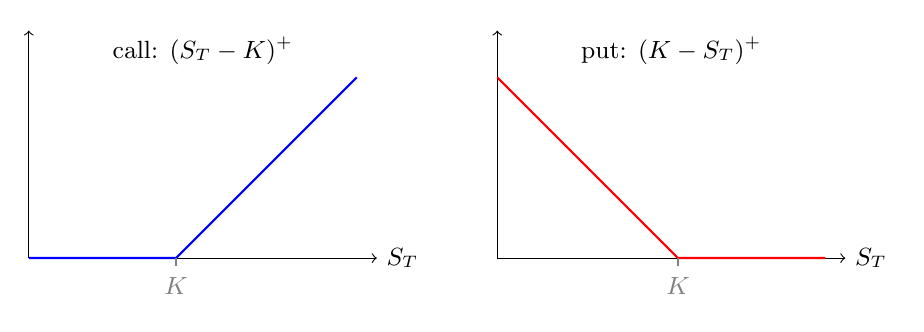
\begin{tikzpicture}[scale=0.85,font=\small]
  \begin{scope}
    \draw[->] (0,0) -- (5.2,0) node[right] {$S_T$};
    \draw[->] (0,0) -- (0,3.4);
    \draw[thick,blue] (0,0) -- (2.2,0) -- (4.9,2.7);
    \draw[dashed,gray] (2.2,0) -- (2.2,-0.15) node[below] {$K$};
    \node at (2.6,3.1) {call: $(S_T-K)^+$};
  \end{scope}
  \begin{scope}[xshift=7cm]
    \draw[->] (0,0) -- (5.2,0) node[right] {$S_T$};
    \draw[->] (0,0) -- (0,3.4);
    \draw[thick,red] (0,2.7) -- (2.7,0) -- (4.9,0);
    \draw[dashed,gray] (2.7,0) -- (2.7,-0.15) node[below] {$K$};
    \node at (2.6,3.1) {put: $(K-S_T)^+$};
  \end{scope}
\end{tikzpicture}
\caption{Payoffs at expiry. Before expiry an option is worth more than this
(it still has \emph{time value}); the surface is about pricing that excess.}
\end{figure}

\subsection{The underlying: an ETF that pays dividends}

\texttt{XIU} holds the 60 largest Canadian stocks and distributes their
dividends, roughly quarterly. Its options are listed on the Montr\'eal Exchange,
expire on the third Friday of the month, and are American-style. Two facts about
the underlying matter for everything that follows: it has a
\emph{spot} price $S$, and it pays \emph{cash dividends} that lower $S$ on the
ex-dividend date. The latter changes both the forward price and the value of
early exercise.

\subsection{What a quote looks like}\label{sec:quotes}

A market maker posts a \emph{bid} (the price at which they buy) and an
\emph{ask} (the price at which they sell). We work with the \emph{mid}
$m=(b+a)/2$, the \emph{spread} $a-b$ and the \emph{relative spread} $(a-b)/m$.
Prices move in \emph{ticks} (here 0.01 CAD). A chain is a table with one row
per contract:

\begin{center}\small
\begin{tabular}{|l|L{9.6cm}|}
\hline
column & meaning \\ \hline
\texttt{expiration}, \texttt{option\_type}, \texttt{strike} & the contract \\ \hline
\texttt{bid}, \texttt{ask} & best prices in CAD per share \\ \hline
\texttt{volume}, \texttt{openInterest} & contracts traded today / outstanding \\ \hline
\texttt{as\_of}, \texttt{spot} & valuation date and underlying price \\ \hline
\end{tabular}
\end{center}

Not every quote is usable. A zero bid means the market maker will not buy at any
price, a very wide relative spread carries little information, and prices at the
one-tick floor reflect the tick size, not volatility. The code keeps a quote only
if $b>0$, $a\ge b$, the mid is finite and $(a-b)/m\le 0.35$; it later also drops
mids below $0.05$ (five ticks). Section~\ref{sec:walkthrough} shows which quotes
these rules remove.

\subsection{Why we invert only out-of-the-money quotes}

For a given strike the market quotes both a call and a put. They are tied by
put-call parity (Section~\ref{sec:parity}), so they carry the same volatility
information. The \emph{out-of-the-money} one (put below the forward, call above)
is the better instrument to read it from: its price is entirely time value, it
is most sensitive to volatility (largest vega per unit of price), and its
early-exercise premium is smallest. The ITM option is mostly intrinsic value
plus the same time value, and for American options it also carries a larger
early-exercise premium.

% ---------------------------------------------------------------------
\section{Pricing by no-arbitrage}\label{sec:pricing}

\subsection{The model}

Fix a probability space with a Brownian motion $W$ under the risk-neutral
measure $\Q$. The ETF price follows geometric Brownian motion with constant
volatility $\sigma$, risk-free rate $r$ and continuous dividend yield $q$:
\begin{equation}\label{eq:gbm}
  dS_t=(r-q)\,S_t\,dt+\sigma S_t\,dW_t .
\end{equation}
By It\^o's formula $d\ln S_t=(r-q-\tfrac12\sigma^2)\,dt+\sigma\,dW_t$, so
\begin{equation}
  S_T=S_0\,e^{(r-q)T}\,\exp\!\bigl(-\tfrac12\sigma^2T+\sigma\sqrt T\,Z\bigr),
  \qquad Z\sim N(0,1).
\end{equation}
The \emph{drift under $\Q$ is $r-q$} because holding the asset earns $q$ in
dividends and, under $\Q$, every tradable total-return asset grows at $r$.

\begin{keyidea}
In a complete, arbitrage-free market the price of a payoff $H$ at $T$ is its
discounted risk-neutral expectation, $V_0=e^{-rT}\E^\Q[H]$. Everything below is
this one formula evaluated for different payoffs and models.
\end{keyidea}

\subsection{The Black--Scholes formula in forward form}\label{sec:bsm}

Define the \emph{forward price} $F=\E^\Q[S_T]=S_0e^{(r-q)T}$ and the discount
factor $D=e^{-rT}$. Then $S_T=F\,e^{-\frac12\sigma^2T+\sigma\sqrt TZ}$ depends on
the rate and the dividends \emph{only through $F$}.

\begin{fact}{Black's formula}
For a European call,
\begin{equation}\label{eq:bsm}
  C=D\,\bigl[F\,\Norm(d_1)-K\,\Norm(d_2)\bigr],\qquad
  d_{1,2}=\frac{\ln(F/K)\pm\tfrac12\sigma^2T}{\sigma\sqrt T},
\end{equation}
and for a put $P=D\,[K\,\Norm(-d_2)-F\,\Norm(-d_1)]$.
\end{fact}

\noindent\emph{Derivation.} Write $C=D\,\E^\Q[(S_T-K)^+]=D\bigl(\E[S_T\mathbf 1_{S_T>K}]-K\,\Q(S_T>K)\bigr)$.
Now $S_T>K$ exactly when $Z>-d_2$, so $\Q(S_T>K)=\Norm(d_2)$. For the first term,
\[
  \E[S_T\mathbf 1_{S_T>K}]=F\int_{-d_2}^{\infty}e^{\sigma\sqrt T z-\frac12\sigma^2T}\,\varphi(z)\,dz
  =F\int_{-d_2}^{\infty}\varphi\bigl(z-\sigma\sqrt T\bigr)\,dz=F\,\Norm(d_2+\sigma\sqrt T)=F\,\Norm(d_1),
\]
where $\varphi$ is the standard normal density; completing the square gives the
shifted density (this is Girsanov's theorem with the asset as numeraire). \hfill$\square$

Working with $(F,D)$ rather than $(S,r,q)$ is the key simplification: a single
formula covers dividends and rates, and (Section~\ref{sec:forward}) the forward
can be read straight from the option market without knowing $q$ at all.

\subsection{Greeks and why volatility can be inverted}

The sensitivities used in the code are taken with respect to $F$ and include $D$.
With $\varphi$ the normal density,
\begin{align}
  \Delta_C&=D\,\Norm(d_1), & \Gamma&=\frac{D\,\varphi(d_1)}{F\sigma\sqrt T}, &
  \mathcal V&=\frac{\partial C}{\partial\sigma}=D\,F\,\varphi(d_1)\sqrt T,\\
  \text{vanna}&=\frac{\partial\Delta}{\partial\sigma}=-\frac{D\varphi(d_1)\,d_2}{\sigma}, &
  \text{volga}&=\frac{\partial\mathcal V}{\partial\sigma}=\frac{\mathcal V\,d_1d_2}{\sigma}.&&
\end{align}
\emph{Vega} $\mathcal V$ is per unit volatility; a one-point move
($\Delta\sigma=0.01$) changes the price by $0.01\,\mathcal V$. Since
$\mathcal V>0$, the price is strictly increasing in $\sigma$, which is what makes
implied volatility well defined (Section~\ref{sec:iv}).

\subsection{Put-call parity and price bounds}\label{sec:parity}

Buy a call and sell a put with the same strike and expiry. At $T$ the payoff is
$(S_T-K)^+-(K-S_T)^+=S_T-K$, the payoff of a forward contract struck at $K$. By
no-arbitrage the two portfolios cost the same today:
\begin{equation}\label{eq:parity}
  C-P=D\,(F-K)\qquad(\text{European}).
\end{equation}
Parity also gives static bounds, which every admissible price must satisfy:
\begin{equation}
  D\max(F-K,0)<C<DF,\qquad D\max(K-F,0)<P<DK.
\end{equation}
A quote outside these bounds is an arbitrage or a data error; the code rejects
it rather than clipping it.

% ---------------------------------------------------------------------
\section{Rates, forwards and dividends}\label{sec:forward}

\subsection{Discounting and the zero curve}

A cash flow at $T$ is discounted by $D(T)=e^{-r(T)\,T}$, where $r(T)$ is the
continuously compounded \emph{zero rate} for maturity $T$. Using the rate of the
option's own maturity, not one flat number, matters when the curve is sloped.
The Bank of Canada publishes (Valet API, open data) six benchmark prints that the
code turns into $r(T)$:

\begin{center}
\begin{center}\small
\begin{tabular}{|l|r|r|r|l|}
\hline
Node & tenor (y) & quoted \% & zero rate \% & print date \\ \hline
CORRA overnight & 0.0027 & 3.30 & 3.2999 & 2025-01-02 \\
1 month T-bill & 0.0833 & 3.19 & 3.1858 & 2025-01-01 \\
3 month T-bill & 0.2500 & 3.16 & 3.1476 & 2025-01-01 \\
6 month T-bill & 0.5000 & 3.09 & 3.0664 & 2025-01-01 \\
1 year T-bill & 1.0000 & 3.03 & 2.9850 & 2025-01-01 \\
2 year bond (par) & 2.0000 & 2.93 & 2.9072 & 2025-01-02 \\
\hline
\end{tabular}
\end{center}

\end{center}

\paragraph{Conversion.} A money-market yield $y$ over tenor $\tau$ is a simple
rate: one dollar grows to $1+y\tau$. The equivalent continuous rate satisfies
$e^{r\tau}=1+y\tau$, i.e.
\begin{equation}
  r=\frac{\ln(1+y\tau)}{\tau}.
\end{equation}

\paragraph{Bootstrapping the 2-year node.} The 2-year benchmark is a
\emph{par yield} $c$: a bond paying coupons $c/2$ every half year at par.
Pricing it at par gives one equation for the unknown 2-year zero rate $r_2$,
\begin{equation}
  \sum_{t\in\{0.5,\,1,\,1.5\}}\frac c2\,e^{-r(t)\,t}+\Bigl(1+\frac c2\Bigr)e^{-2r_2}=1,
\end{equation}
where $r(0.5),r(1)$ come from the shorter nodes and $r(1.5)$ is linear between
$r(1)$ and $r_2$. The result (2.907\% against 2.909\% if the par yield were used
directly) shows the shortcut would have been harmless here, but the code does
the bootstrap. Between nodes $r(T)$ is linear in the tenor and beyond the
last node it is flat.

\subsection{Forward price, dividends and the cost of carry}

Holding the asset until $T$ costs interest on the price and forgoes nothing but
earns dividends, so the no-arbitrage forward is
\begin{equation}\label{eq:forward}
  F=S\,e^{(r-q)T}\quad(\text{continuous yield}),\qquad
  F=\bigl(S-\mathrm{PV}(\text{dividends before }T)\bigr)e^{rT}\quad(\text{discrete}),
\end{equation}
where $\mathrm{PV}(\cdot)=\sum_i d_i e^{-r t_i}$ discounts each cash dividend
$d_i$ paid at $t_i$. The discrete form is the \emph{escrowed dividend} model: the
dividends already declared are set aside, and only the remainder $S-\mathrm{PV}$
is risky. For a given $F$, the two forms are linked by the \emph{implied yield}
\begin{equation}
  q=r-\frac{\ln(F/S)}{T}.
\end{equation}

\subsection{Reading the forward from the option market}

Rearranging parity~\eqref{eq:parity} for a strike with both a call and a put gives
a forward estimate that uses no model at all:
\begin{equation}\label{eq:fhat}
  \hat F_i=K_i+\frac{C_i-P_i}{D(T)}.
\end{equation}
The code takes the three strikes closest to the spot and uses the \emph{median}
of their $\hat F_i$, which is robust to one noisy pair. There is no fallback to
$Se^{rT}$: ignoring dividends there would silently bias every vol, so an expiry
without a call/put pair is dropped. (For American options \eqref{eq:parity} is
only a bound, which is why the code corrects it; see
Section~\ref{sec:am-parity}.)

% ---------------------------------------------------------------------
\section{American options}\label{sec:american}

\subsection{Early exercise as optimal stopping}

An American option is worth
\begin{equation}
  V_0=\sup_{\tau\le T}\E^\Q\bigl[e^{-r\tau}\,\mathrm{payoff}(S_\tau)\bigr],
\end{equation}
the best discounted expected payoff over all stopping times, so it is at least a
European option and at least its intrinsic value:
$V_A\ge V_E$ and $V_A\ge\mathrm{payoff}(S_0)$. The difference
$\mathrm{premium}=V_A-V_E\ge0$ is the \emph{early-exercise premium}. There is no
closed form in general; the value is found numerically.

\subsection{When is exercising early worth it?}

\begin{fact}{No early exercise of a call without dividends}
If $q=0$ and $r\ge0$, an American call is never exercised before $T$, so
$C_A=C_E$.
\end{fact}

\noindent\emph{Why.} A European call satisfies $C_E\ge S-KD>S-K$ for $r>0$:
holding is always worth more than exercising, because exercising forfeits both
the interest on $K$ and the optionality. \hfill$\square$

Two things break this. For a \emph{put}, a deep in-the-money option can be worth
exercising to earn interest on the strike. For a \emph{call}, an imminent
dividend lowers the price on the ex-date, so it can pay to exercise just
\emph{before} it. Figure~\ref{fig:premium} shows both effects.

\begin{figure}[ht]
\centering
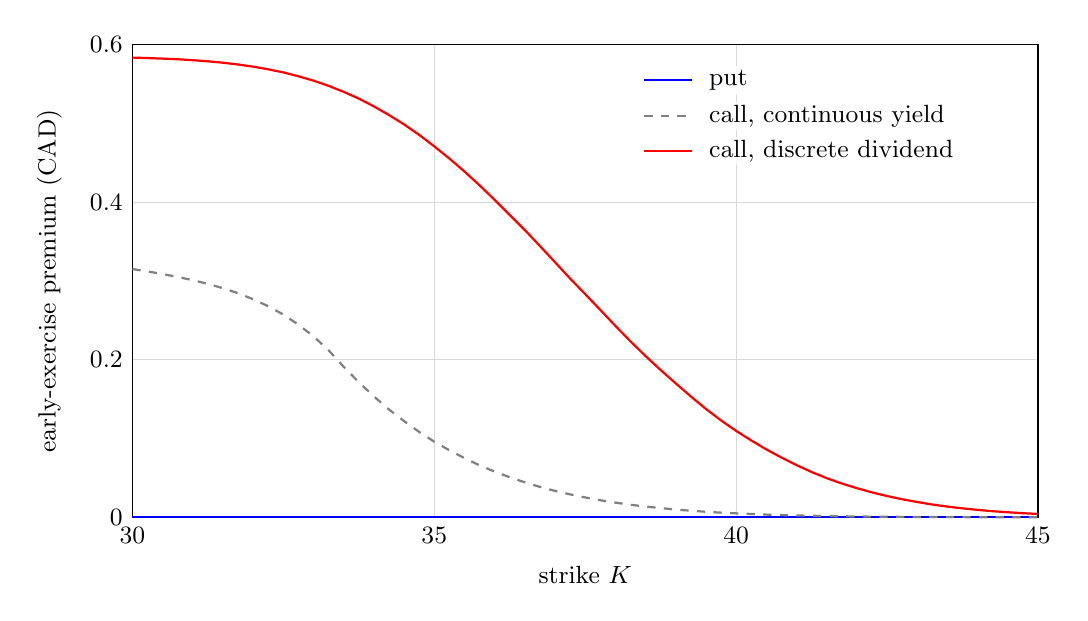
\begin{tikzpicture}[font=\small]
\draw[gray!30] (0.000,0) -- (0.000,6.0);
\node[below] at (0.000,0) {30};
\draw[gray!30] (3.833,0) -- (3.833,6.0);
\node[below] at (3.833,0) {35};
\draw[gray!30] (7.667,0) -- (7.667,6.0);
\node[below] at (7.667,0) {40};
\draw[gray!30] (11.500,0) -- (11.500,6.0);
\node[below] at (11.500,0) {45};
\draw[gray!30] (0,0.000) -- (11.5,0.000);
\node[left] at (0,0.000) {0};
\draw[gray!30] (0,2.000) -- (11.5,2.000);
\node[left] at (0,2.000) {0.2};
\draw[gray!30] (0,4.000) -- (11.5,4.000);
\node[left] at (0,4.000) {0.4};
\draw[gray!30] (0,6.000) -- (11.5,6.000);
\node[left] at (0,6.000) {0.6};
\draw (0,0) rectangle (11.5,6.0);
\node[below=14pt] at (5.75,0) {strike $K$};
\node[rotate=90,above=22pt] at (0,3.0) {early-exercise premium (CAD)};
\draw[blue,thick] plot coordinates {(0.000,0.000) (0.192,0.000) (0.383,0.000) (0.575,0.000) (0.767,0.000) (0.958,0.000) (1.150,0.000) (1.342,0.000) (1.533,0.000) (1.725,0.000) (1.917,0.000) (2.108,0.000) (2.300,0.000) (2.492,0.000) (2.683,0.000) (2.875,0.000) (3.067,0.000) (3.258,0.000) (3.450,0.000) (3.642,0.000) (3.833,0.000) (4.025,0.000) (4.217,0.000) (4.408,0.000) (4.600,0.000) (4.792,0.000) (4.983,0.000) (5.175,0.000) (5.367,0.000) (5.558,0.000) (5.750,0.000) (5.942,0.000) (6.133,0.000) (6.325,0.000) (6.517,0.000) (6.708,0.000) (6.900,0.000) (7.092,0.000) (7.283,0.000) (7.475,0.000) (7.667,0.000) (7.858,0.000) (8.050,0.000) (8.242,0.000) (8.433,0.000) (8.625,0.000) (8.817,0.000) (9.008,0.000) (9.200,0.000) (9.392,0.000) (9.583,0.000) (9.775,0.000) (9.967,0.000) (10.158,0.000) (10.350,0.000) (10.542,0.000) (10.733,0.000) (10.925,0.000) (11.117,0.000) (11.308,0.000) (11.500,0.000)};
\draw[gray,thick,dashed] plot coordinates {(0.000,3.153) (0.192,3.123) (0.383,3.090) (0.575,3.053) (0.767,3.012) (0.958,2.965) (1.150,2.910) (1.342,2.846) (1.533,2.770) (1.725,2.681) (1.917,2.575) (2.108,2.447) (2.300,2.298) (2.492,2.121) (2.683,1.911) (2.875,1.716) (3.067,1.535) (3.258,1.370) (3.450,1.222) (3.642,1.085) (3.833,0.961) (4.025,0.852) (4.217,0.752) (4.408,0.661) (4.600,0.581) (4.792,0.509) (4.983,0.445) (5.175,0.387) (5.367,0.336) (5.558,0.292) (5.750,0.253) (5.942,0.217) (6.133,0.187) (6.325,0.160) (6.517,0.137) (6.708,0.118) (6.900,0.099) (7.092,0.084) (7.283,0.071) (7.475,0.060) (7.667,0.051) (7.858,0.043) (8.050,0.035) (8.242,0.029) (8.433,0.024) (8.625,0.020) (8.817,0.017) (9.008,0.014) (9.200,0.011) (9.392,0.009) (9.583,0.008) (9.775,0.006) (9.967,0.005) (10.158,0.004) (10.350,0.003) (10.542,0.003) (10.733,0.002) (10.925,0.002) (11.117,0.001) (11.308,0.001) (11.500,0.001)};
\draw[red,thick] plot coordinates {(0.000,5.839) (0.192,5.833) (0.383,5.826) (0.575,5.818) (0.767,5.806) (0.958,5.792) (1.150,5.774) (1.342,5.751) (1.533,5.724) (1.725,5.690) (1.917,5.651) (2.108,5.602) (2.300,5.546) (2.492,5.480) (2.683,5.404) (2.875,5.318) (3.067,5.219) (3.258,5.110) (3.450,4.990) (3.642,4.857) (3.833,4.712) (4.025,4.557) (4.217,4.392) (4.408,4.217) (4.600,4.032) (4.792,3.840) (4.983,3.649) (5.175,3.446) (5.367,3.240) (5.558,3.033) (5.750,2.835) (5.942,2.634) (6.133,2.432) (6.325,2.235) (6.517,2.048) (6.708,1.871) (6.900,1.701) (7.092,1.535) (7.283,1.377) (7.475,1.231) (7.667,1.098) (7.858,0.977) (8.050,0.863) (8.242,0.760) (8.433,0.664) (8.625,0.576) (8.817,0.498) (9.008,0.430) (9.200,0.371) (9.392,0.317) (9.583,0.271) (9.775,0.230) (9.967,0.195) (10.158,0.163) (10.350,0.137) (10.542,0.114) (10.733,0.095) (10.925,0.078) (11.117,0.065) (11.308,0.053) (11.500,0.043)};
\fill[white,opacity=0.85] (6.3,5.37) rectangle (11.4,5.7299999999999995);
\draw[blue,thick] (6.5,5.55) -- (7.1,5.55);
\node[right] at (7.2,5.55) {put};
\fill[white,opacity=0.85] (6.3,4.92) rectangle (11.4,5.279999999999999);
\draw[gray,thick,dashed] (6.5,5.1) -- (7.1,5.1);
\node[right] at (7.2,5.1) {call, continuous yield};
\fill[white,opacity=0.85] (6.3,4.47) rectangle (11.4,4.829999999999999);
\draw[red,thick] (6.5,4.6499999999999995) -- (7.1,4.6499999999999995);
\node[right] at (7.2,4.6499999999999995) {call, discrete dividend};
\end{tikzpicture}

\caption{Early-exercise premium by strike ($S=37.70$, $T=0.31$, $\sigma=14\%$,
$r=3\%$; a 0.60 CAD dividend 0.30 years out). Puts gain value as they go deep in
the money. A call has a negligible premium if the dividend is smoothed into a
yield, but a visible one if it is a discrete payment just before expiry.}
\label{fig:premium}
\end{figure}

\subsection{Put-call parity is only a bound}\label{sec:am-parity}

For American options, with $\Delta=\mathrm{PV}(\text{dividends})$,
\begin{equation}
  S-\Delta-K\ \le\ C_A-P_A\ \le\ S-KD.
\end{equation}
The European value $D(F-K)$ lies inside this interval but the American difference
need not equal it. Using \eqref{eq:fhat} on American mids therefore biases the
forward whenever the call or the put carries early-exercise value, most of all
for an expiry that coincides with an ex-dividend date. The correction in
Section~\ref{sec:fcorr} removes that bias.

\subsection{The binomial tree (Cox--Ross--Rubinstein)}\label{sec:crr}

Divide $[0,T]$ into $n$ steps of length $\Delta t$. In each step the price moves
to $uS$ or $dS$ with $u=e^{\sigma\sqrt{\Delta t}}$ and $d=1/u$. Choosing the
risk-neutral up-probability $p$ so that the one-step mean matches the continuous
model, $p\,u+(1-p)\,d=e^{(r-q)\Delta t}$, gives
\begin{equation}
  p=\frac{e^{(r-q)\Delta t}-d}{u-d}.
\end{equation}
The one-step variance then tends to $\sigma^2\Delta t$, so by the central limit
theorem the terminal price converges to the lognormal law of
Section~\ref{sec:bsm}. Option values follow by backward induction from the
terminal payoff, with the right to exercise early added at every node:
\begin{equation}\label{eq:tree}
  V_{i,j}=\max\!\Bigl(\mathrm{payoff}(S_{i,j}),\ e^{-r\Delta t}\bigl[p\,V_{i+1,j+1}+(1-p)\,V_{i+1,j}\bigr]\Bigr).
\end{equation}
For a European option drop the $\max$. The tree needs $p\in(0,1)$, i.e.
$\sigma\sqrt{\Delta t}>|r-q|\Delta t$, which constrains the lowest volatility it
can represent. Trees oscillate with the parity of $n$, so the code averages the
values from $n$ and $n+1$ steps.

\begin{figure}[ht]
\centering
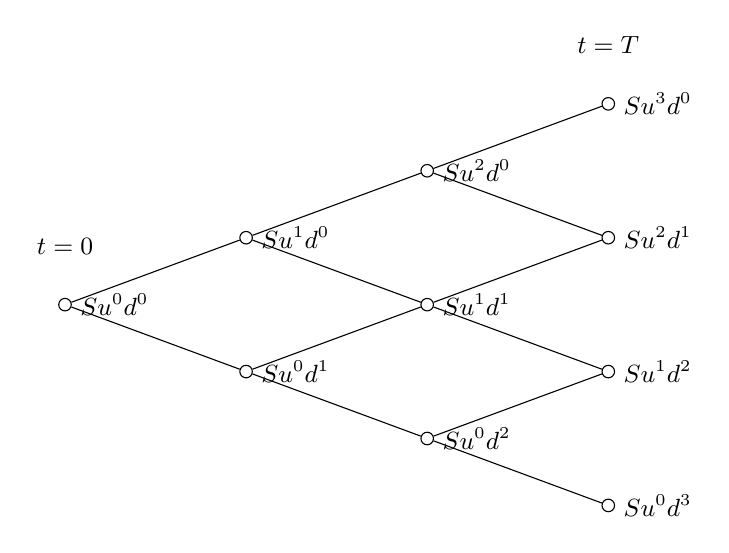
\begin{tikzpicture}[x=2.3cm,y=0.85cm,font=\small]
  \foreach \i in {0,...,3}{
    \foreach \j in {0,...,\i}{
      \pgfmathtruncatemacro{\a}{\i-\j}
      \node[circle,draw,inner sep=1.6pt] (n\i\j) at (\i,{\i-2*\j}) {};
      \node[right=2pt] at (n\i\j) {$Su^{\a}d^{\j}$};
    }
  }
  \foreach \i in {0,...,2}{
    \foreach \j in {0,...,\i}{
      \pgfmathtruncatemacro{\ii}{\i+1}
      \pgfmathtruncatemacro{\jj}{\j+1}
      \draw (n\i\j) -- (n\ii\j);
      \draw (n\i\j) -- (n\ii\jj);
    }
  }
  \node[above] at (0,0.6) {$t=0$};
  \node[above] at (3,3.6) {$t=T$};
\end{tikzpicture}
\caption{A three-step recombining tree. At every node the holder compares the
payoff from exercising now with the discounted expected value of continuing,
equation~\eqref{eq:tree}.}
\end{figure}

\subsection{Discrete dividends in the tree}

Two ways to realise dividends, with the same forward.

\paragraph{Continuous yield.} Run the tree on $S$ with drift $r-q$, where $q$ is
the yield implied by the forward. This needs no schedule, but spreads the
dividend over the whole life.

\paragraph{Escrowed discrete dividends.} Run the tree on the dividend-free
price $S^*=Se^{-qT}$ (drift $r$) and value early exercise at time $t$ on
$S^*_t+\mathrm{PV}_t$, where $\mathrm{PV}_t$ is the value at $t$ of the
dividends still to be paid before expiry. The schedule only times the
dividends: $\mathrm{PV}_0$ is rescaled to equal $S-S^*$, so the forward is
unchanged. A call is then worth most just before an ex-date. (A schedule more
than twice off the forward is ignored in favour of the continuous yield.)

\subsection{The cost of ignoring early exercise}

Suppose a quote is the American price at the true volatility $\sigma$, but we
invert it with a European model to get $\sigma_E$. Then
$V_E(\sigma_E)=V_A(\sigma)=V_E(\sigma)+\mathrm{premium}$, and to first order
\begin{equation}\label{eq:bias}
  \sigma_E-\sigma\ \approx\ \frac{\mathrm{premium}}{\mathcal V}.
\end{equation}
A European inversion therefore \emph{overstates} volatility by premium over vega.
The code reports this number for every slice in both modes.

% ---------------------------------------------------------------------
\section{Implied volatility and the smile}\label{sec:smile}

\subsection{Definition and inversion}\label{sec:iv}

\begin{defn}{Implied volatility}
For a quote $m$, the implied volatility $\sigma_{\mathrm{imp}}$ is the number for
which the model price equals $m$: $\mathrm{Price}(\sigma_{\mathrm{imp}})=m$.
\end{defn}

Existence and uniqueness follow from two facts. The price is strictly increasing
in $\sigma$ (positive vega), and it ranges over exactly the no-arbitrage interval
as $\sigma$ goes from 0 to $\infty$. So a root exists iff $m$ is strictly inside
the bounds, and then it is unique. The code finds it with Brent's method on
$[10^{-5},5]$ for the European model and with a safeguarded Newton iteration on
the tree for the American one (the European vega is used as the slope, with a
bisection fallback). Quotes at or outside the bounds are skipped and counted,
never clipped.

\subsection{The smile}

If Black--Scholes were true, $\sigma_{\mathrm{imp}}$ would be the same for every
strike and expiry. It is not. Plotted against strike, equity-index implied
volatility typically slopes down (a \emph{skew}: downside protection is
expensive), and it varies with maturity (a \emph{term structure}). It is
convenient to work with \emph{total variance} $w=\sigma^2T$ and log-moneyness
$k=\ln(K/F)$, because arbitrage conditions become simple statements about
$w(k,T)$.

\subsection{Parametrizing one slice: raw SVI}\label{sec:svi-theory}

Market quotes are a scattering of points. The surface needs a smooth function, so
each expiry is fitted with Gatheral's \emph{raw SVI}:
\begin{equation}\label{eq:svi}
  w(k)=a+b\Bigl[\rho\,(k-m)+\sqrt{(k-m)^2+s^2}\Bigr],
\end{equation}
with $a$ the overall level, $b$ the angle between the wings, $\rho\in(-1,1)$ the
skew (rotation), $m$ the horizontal shift and $s>0$ the smoothing of the vertex.
It is a hyperbola: linear in the wings, as Lee's moment formula requires
(total variance cannot grow faster than $2|k|$), and curved near the money.
Admissible parameters satisfy $b\ge0$, $|\rho|<1$, $s>0$ and a nonnegative
minimum variance
\begin{equation}
  a+b\,s\sqrt{1-\rho^2}\ \ge\ 0 .
\end{equation}

\subsection{Static arbitrage: butterflies and calendars}

A surface that cannot be traded against must have a non-negative risk-neutral
density in strike and non-decreasing option value in maturity.

\begin{fact}{Butterfly condition (Durrleman)}
The density of $S_T$ implied by a slice $w(k)$ is
$\dfrac{g(k)}{\sqrt{2\pi w}}\,e^{-d_-^2/2}$ with $d_-=-k/\sqrt w-\sqrt w/2$, where
\begin{equation}\label{eq:g}
  g(k)=\Bigl(1-\frac{k\,w'}{2w}\Bigr)^2-\frac{w'^2}{4}\Bigl(\frac1w+\frac14\Bigr)+\frac{w''}{2}.
\end{equation}
So the slice admits no butterfly arbitrage iff $g(k)\ge0$ for all $k$.
\end{fact}

A \emph{butterfly spread} (long two options at $K$, short one each at $K\pm\delta$)
has a non-negative payoff, so its price must be non-negative; in the limit
$\delta\to0$ this says $\partial^2C/\partial K^2\ge0$ (Breeden--Litzenberger),
which is positivity of the density above.

\begin{fact}{Calendar condition}
There is no calendar-spread arbitrage iff, for every $k$,
$\partial w(k,T)/\partial T\ge0$: total variance cannot fall with maturity.
\end{fact}

\paragraph{SSVI: arbitrage-free by construction.} Gatheral and
Jacquier's SSVI parametrizes the whole surface with an ATM total variance
$\theta(T)=\sigma_{\mathrm{atm}}(T)^2T$ and a curvature function
$\varphi(\theta)=\eta\,\theta^{-\gamma}$:
\begin{multline}\label{eq:ssvi}
  w(k,T)=\frac\theta2\Bigl(1+\rho\,\varphi k\\
  +\sqrt{(\varphi k+\rho)^2+1-\rho^2}\Bigr).
\end{multline}
Each slice is exactly a raw SVI (with $a=\tfrac\theta2(1-\rho^2)$,
$b=\tfrac{\theta\varphi}2$, $m=-\rho/\varphi$, $s=\sqrt{1-\rho^2}/\varphi$), and the
surface is free of both arbitrages if $\theta$ is increasing,
$\theta\varphi(1+|\rho|)<4$, $\theta\varphi^2(1+|\rho|)\le4$ and
$0\le\partial_\theta(\theta\varphi)\le\frac{1+\sqrt{1-\rho^2}}{\rho^2}\,\varphi$. The
project uses SSVI only to \emph{generate} its synthetic market
(Section~\ref{sec:synthetic}); the pipeline then fits ordinary raw SVI to the
noisy quotes and must find a surface that is again arbitrage-free.

% =====================================================================
\part{The algorithm}
% =====================================================================

\section{Architecture and data model}\label{sec:arch}

The data flow is a straight line from quotes to a JSON file, with the pricing
model as the only switch.

\begin{center}\small
\begin{tabular}{|L{3.4cm}|L{11.2cm}|}
\hline
Module & Role \\ \hline
\texttt{synthetic.py} & the generated chain (SSVI truth, American prices, tick-sized quotes) \\ \hline
\texttt{rates.py} & Bank of Canada curve, bootstrap, JSON snapshots \\ \hline
\texttt{data.py} & quote filter, per-expiry rate, parity forward (with an optional mid adjustment) \\ \hline
\texttt{bsm.py} & forward Black--Scholes price, Greeks, Brent inversion (European) \\ \hline
\texttt{american.py} & CRR tree, discrete dividends, Newton inversion, early-exercise premium \\ \hline
\texttt{svi.py} & raw SVI, constrained fit, butterfly and calendar checks \\ \hline
\texttt{surface.py} & the pipeline, mesh, JSON writer and command line \\ \hline
\texttt{api.py}, \texttt{static/} & file-backed API and the interactive 3D page \\ \hline
\end{tabular}
\end{center}

The pipeline never repairs bad data. It \emph{counts} skipped quotes (below the
mid floor, outside the arbitrage bounds, no root), \emph{lists} rejected expiries
with their reason, and \emph{reports} a failed calendar check, so the output is
honest about what it could and could not fit.

\section{The algorithm in pseudo-code}\label{sec:algo}

\begin{algobox}{Algorithm 1: BuildSurface}
\begin{verbatim}
input : chain, spot S, rate curve r(.), exercise in {european, american},
        dividends (optional schedule)
output: surface document

 1. clean <- FilterQuotes(chain)               # b>0, a>=b, spread<=35%
 2. for each row: T <- days/365, r <- r(T), D <- exp(-r*T)
 3. F <- ParityForward(clean)                  # Algorithm 2, per expiry
 4. if exercise = american:
 5.     repeat 3 times:
 6.         prem <- EarlyExercisePremium(clean rows within 6% of F)
 7.         F <- ParityForward(clean, mid - prem)    # corrected forward
 8. otm <- rows with (put and K<F) or (call and K>=F), and mid >= 0.05
 9. sigma <- Invert(otm)                       # Algorithm 3; count failures
10. for each expiry:
11.     if fewer than 5 usable quotes: reject, record the reason
12.     else: params <- FitSVI(k=ln(K/F), w=sigma^2*T)   # Algorithm 4
13.            on failure: reject, record the reason
14. check dw/dT >= 0 across fitted expiries    # report, never repair
15. mesh <- 6 interpolated rows between expiries (linear in w; no
                                                       extrapolation)
16. write surface atomically as JSON
\end{verbatim}
\end{algobox}

\begin{algobox}{Algorithm 2: ParityForward (one expiry)}
\begin{verbatim}
input : mids of calls C(K), puts P(K), discount D, spot S
output: forward F

1. pairs <- strikes K that have both a call and a put
2. for each pair: Fhat <- K + (C - P)/D            # equation (fhat)
3. near <- the 3 pairs with smallest |K - S|
4. return median of Fhat over near
\end{verbatim}
\end{algobox}

\begin{algobox}{Algorithm 3: Invert (mids to implied volatilities)}
\begin{verbatim}
european : for each row, if D*max(F-K,0) < m < D*F (call) or the put bounds:
               sigma <- Brent root of BSM(sigma) - m on [1e-5, 5]
           else count as arbitrage_bounds; no root -> solver_bracket
american : for each (expiry, side), q <- r - ln(F/S)/T
               prices outside (intrinsic, S or K)   -> NaN, counted
               sigma0 <- 0.2
               repeat up to 40 times:
                   err <- TreePrice(sigma) - m      # all strikes at once
                   narrow the bracket [lo, hi] using sign(err)
                   sigma <- sigma - err / vega_BSM  # Newton step
                   if the step leaves [lo, hi]: sigma <- (lo + hi)/2
                   stop when max |change| < 1e-9
\end{verbatim}
\end{algobox}

\begin{algobox}{Algorithm 4: FitSVI (one expiry)}
\begin{verbatim}
input : points (k_i, w_i), i = 1..n  with n >= 5
output: parameters (a, b, rho, m, s)

1. grid <- the k_i plus 201 points on [min k - 0.5, max k + 0.5]
2. minimize  sum_i (w(k_i) - w_i)^2 / mean(w)^2        # SLSQP, ftol 1e-10
     subject to  b >= 0,  |rho| <= 1-1e-6,  s >= 1e-6,
                 a + b*s*sqrt(1-rho^2) >= 0,
                 g(k) >= 0 for every k in grid                (equation g)
3. start from rho0 in {-0.5, 0, 0.5} (a0 = min(w)/2, b0 = range(w)/range(k),
   m0 = argmin w, s0 = 0.1); keep the converged run with lowest objective
4. if no run converged, or g(k) < 0 anywhere on the grid: reject (no clamp)
\end{verbatim}
\end{algobox}

\begin{algobox}{Algorithm 5: TreePrice (CRR with escrowed dividends)}
\begin{verbatim}
input : S, K, T, r, q, sigma, side, steps n, optional dividend schedule
 1. dt <- T/n;  u <- exp(sigma*sqrt(dt));  d <- 1/u
 2. p <- (exp((r-q)*dt) - d)/(u - d);  require 0 < p < 1
 3. if a schedule applies: S* <- S*exp(-q*T), drift <- r,
        owed_t <- schedule PV at each level, rescaled so owed_0 = S - S*
    else: S* <- S, drift <- r - q, owed_t <- 0
 4. V[n, j] <- payoff(S* u^(2j-n))                    # terminal nodes
 5. for level i = n-1 down to 0:
        V[i, j] <- exp(-r*dt) * (p*V[i+1, j+1] + (1-p)*V[i+1, j])
        V[i, j] <- max(V[i, j], payoff(S* u^(2j-i) + owed_i))   # American
 6. return V[0, 0]      # the code averages the n-step and (n+1)-step trees
\end{verbatim}
\end{algobox}

\paragraph{Complexity.} A tree costs $O(n^2)$ per option, but all strikes of one
expiry and side share the same tree shape, so they are priced in one vectorized
array. With $n=200$ the whole demo (780 quotes in, 633 past the quality
filter, 240 out-of-the-money quotes inverted over 12 fitted expiries, plus three
forward-correction passes) takes about ten seconds; the European variant takes
about five.

\section{The variants and the defaults}\label{sec:choice}

Two switches control how mids become volatilities. \texttt{--exercise} picks the
pricing model and \texttt{--dividends} picks how the American tree realises
dividends.

\begin{center}\small
\begin{tabular}{|L{3.1cm}|L{5.6cm}|L{5.8cm}|}
\hline
 & \texttt{european} & \texttt{american} (default) \\ \hline
Price & closed-form forward BSM, equation~\eqref{eq:bsm} & CRR tree with early exercise, \eqref{eq:tree} \\ \hline
Module and solver & \texttt{bsm.py}, Brent, one quote at a time & \texttt{american.py}, safeguarded Newton, vectorized per expiry and side \\ \hline
Forward & raw put-call parity & parity corrected for early exercise (3 passes) \\ \hline
Extra inputs & none & implied yield $q$, optionally a dividend schedule \\ \hline
Demo run time & about 5\,s & about 10\,s \\ \hline
Mean ATM error vs truth & \atmErrEuropean\ vol points (worst \atmWorstEuropean) & \atmErrAmerican\ (worst \atmWorstAmerican) \\ \hline
\end{tabular}
\end{center}

\texttt{american} is the default because \texttt{XIU} options \emph{are}
American-style, and by \eqref{eq:bias} the European model overstates their
volatility. \texttt{european} is kept for speed and as the baseline that shows how
much early exercise matters; both modes still record the premium and bias of every
slice.

\begin{center}\small
\begin{tabular}{|L{3.1cm}|L{5.6cm}|L{5.8cm}|}
\hline
 & \texttt{schedule} & \texttt{continuous} \\ \hline
Dividends & discrete cash payments at known dates & a smooth yield $q$ over the life \\ \hline
Exercise valued on & $S^*+\mathrm{PV}_t$ & $S$ \\ \hline
Call before an ex-date & worth most & understated \\ \hline
Default & the demo (it knows its own schedule) & any run without a schedule \\ \hline
\end{tabular}
\end{center}

The demo's generating process pays discrete dividends, so the schedule recovers
the truth and the continuous yield overstates ATM volatility (mean error
\atmErrContinuous\ vol points); a test asserts that the schedule's error is less
than half of the continuous one's.

\subsection{Correcting the forward for early exercise}\label{sec:fcorr}

Parity \eqref{eq:parity} is a European identity, so on American mids the estimate
\eqref{eq:fhat} is biased. The fix subtracts each near-the-money quote's own
premium before applying parity. After a first estimate, the premium of every quote
within 6\% of the forward is computed at its European volatility (Section
\ref{sec:american}) and subtracted from its mid, and the forward is re-estimated;
three passes converge. On the demo this cuts the forward error on the expiry that
falls on an ex-date from 0.33\% to about 0.01\% of $F$.

\section{Numerical details and safeguards}\label{sec:numerics}

\begin{itemize}
  \item \textbf{Reject, do not repair.} Quotes outside the arbitrage bounds,
        expiries whose fit violates $g\ge0$, and a failed calendar check are
        reported with a reason. Nothing is clipped into apparent validity.
  \item \textbf{Constraints, not penalties.} Butterfly freedom is imposed as a
        constraint of the SVI fit on a grid that extends well beyond the quotes
        (0.5 in $k$), then re-checked on the same grid.
  \item \textbf{Tree validity.} The probability $p$ must lie in $(0,1)$; the
        inversion therefore starts above a floor $\sigma>|r-q|\sqrt{\Delta t}$.
  \item \textbf{Local optimizer.} SLSQP with three starts is a local, not a global,
        method. On the demo one thin expiry (8 quotes, on an ex-date) can be
        rejected on some platforms; it is then reported, not repaired.
  \item \textbf{Determinism.} The synthetic chain uses a fixed seed. Tests are
        offline, and live data is only fetched with an explicit flag, at one
        request per expiry, with a pause, no retries and a 30-minute cooldown.
  \item \textbf{Atomic output.} The JSON is written to a temporary file and
        renamed, so the API never reads a partial file; non-finite numbers become
        \texttt{null}.
\end{itemize}

% =====================================================================
\part{A worked example}
% =====================================================================

\section{The synthetic market}\label{sec:synthetic}

Because no real quotes are available the market is generated, in three stages.

\paragraph{1. A truth surface.} The true surface is the SSVI
\eqref{eq:ssvi} with ATM volatility $\sigma_{\mathrm{atm}}(T)$ rising from
11.5\% to 13.5\% (the realized volatility of \texttt{XIU.TO} was 8.8--10.9\% in
January 2025), $\rho=-0.65$, $\eta=0.9$ and $\gamma=0.4$. The code verifies the
SSVI conditions of Section~\ref{sec:smile} on $(0,3]$ years and tests that every
slice has $g\ge0$. A 3-month 90\%-moneyness put then trades about 3.5 vol points
above the ATM level, a realistic index skew.

\paragraph{2. Real inputs.} Spot (37.70) and the four trailing quarterly
dividends come from one free Yahoo history request (derived statistics only, no
price series stored); the next year's dividends are the same four, shifted by
364 days. The risk-free curve is the Bank of Canada snapshot above.

\paragraph{3. American prices and tick-sized quotes.} For every third-Friday
expiry and strike, the option is priced with the discrete-dividend American tree
at the \emph{truth} volatility. The mid is then perturbed by a seeded random
shift of up to a quarter spread, and bid and ask are placed around it with a
spread of $\max(0.02,\,5\%\text{ of the mid})$, rounded outwards to the 0.01
tick; bids that round to zero are zero. This gives 780 quotes over 13 expiries,
with the same kinds of defects as a real chain (wide spreads far out of the money,
zero bids, thin volume).

\noindent The pipeline thus faces exactly the effect it must undo: the quotes are
American and the dividends discrete. (An earlier version priced and inverted with
the same continuous-yield tree, which hid the bias that Section~\ref{sec:results}
now measures.)

\section{Walkthrough: one expiry, step by step}\label{sec:walkthrough}

We follow the expiry of \textbf{21 March 2025} ($T=0.2137$ years, 78 days after the
valuation date 2 January 2025, spot $S=37.70$).

\subsection{The raw quotes}

Table below shows the strikes around the money. Each row is a strike; the left
block is the call and the right block the put. A star marks a quote the filter
removes: zero bid, or a relative spread above 35\%.

\begin{center}\small
\begin{tabular}{|r|rrrr|rrrr|}
\hline
K & bid & ask & mid & spr. & bid & ask & mid & spr. \\ \hline
35.0 & 2.88 & 3.04 & 2.960 & 5\% & 0.16 & 0.19 & 0.175 & 17\% \\
35.5 & 2.43 & 2.56 & 2.495 & 5\% & 0.23 & 0.26 & 0.245 & 12\% \\
36.0 & 2.03 & 2.14 & 2.085 & 5\% & 0.30 & 0.33 & 0.315 & 10\% \\
36.5 & 1.63 & 1.73 & 1.680 & 6\% & 0.43 & 0.46 & 0.445 & 7\% \\
37.0 & 1.28 & 1.36 & 1.320 & 6\% & 0.57 & 0.61 & 0.590 & 7\% \\
37.5 & 0.95 & 1.01 & 0.980 & 6\% & 0.75 & 0.80 & 0.775 & 6\% \\
38.0 & 0.69 & 0.73 & 0.710 & 6\% & 0.96 & 1.02 & 0.990 & 6\% \\
38.5 & 0.46 & 0.49 & 0.475 & 6\% & 1.24 & 1.32 & 1.280 & 6\% \\
39.0 & 0.28 & 0.31 & 0.295 & 10\% & 1.57 & 1.66 & 1.615 & 6\% \\
39.5 & 0.15 & 0.18 & 0.165 & 18\% & 1.96 & 2.07 & 2.015 & 5\% \\
40.0 & 0.07 & 0.10 & 0.085\textsuperscript{*} & 35\% & 2.36 & 2.49 & 2.425 & 5\% \\
40.5 & 0.03 & 0.06 & 0.045\textsuperscript{*} & 67\% & 2.81 & 2.96 & 2.885 & 5\% \\
41.0 & 0.00 & 0.03 & 0.015\textsuperscript{*} & 200\% & 3.29 & 3.47 & 3.380 & 5\% \\
\hline
\end{tabular}
\end{center}


The full expiry has \nRaw\ quotes and \nPass\ survive the filter; the rest are
far-out-of-the-money options priced at a few ticks, where the spread is a large
fraction of the price.

\subsection{Rate, discount and forward}

At $T=0.2137$ the curve gives $r=3.156\%$ and $D=e^{-rT}=0.9933$. The forward
from the three at-the-money pairs, equation~\eqref{eq:fhat}:

\begin{center}\small
\begin{tabular}{|r|r|r|r|}
\hline
K & call mid & put mid & $\hat F=K+(C-P)/D$ \\ \hline
37.0 & 1.3200 & 0.5900 & 37.7349 \\
37.5 & 0.9800 & 0.7750 & 37.7064 \\
38.0 & 0.7100 & 0.9900 & 37.7181 \\
\hline
\end{tabular}
\end{center}


The median is $37.718$. The three estimates disagree by about 3 cents, a hint of
the noise the median guards against. They also carry a systematic error: the
mids are American. Subtracting each pair's early-exercise premium (Section
\ref{sec:fcorr}) moves the forward to $37.708$, $37.705$ and $37.704$ over the
three passes. The generating forward is $37.7005$, so the raw estimate was
1.8 cents (0.05\%) too high and the corrected one is 0.4 cents (0.01\%) off.

\subsection{Implied volatilities, two ways}

Only out-of-the-money quotes are inverted (puts below $F=37.70$, calls above).
$\sigma_E$ treats the mid as a European price; $\sigma_A$ inverts it with the
American tree and the dividend schedule; the last column is the true volatility
from the generating surface.

\begin{center}\small
\begin{tabular}{|r|l|r|r|r|r|}
\hline
K & side & mid & $\sigma_E$ \% & $\sigma_A$ \% & truth \% \\ \hline
34.0 & put & 0.095 & 15.93 & 15.88 & 15.69 \\
34.5 & put & 0.125 & 15.25 & 15.19 & 15.21 \\
35.0 & put & 0.175 & 14.84 & 14.78 & 14.73 \\
35.5 & put & 0.245 & 14.50 & 14.41 & 14.24 \\
36.0 & put & 0.315 & 13.71 & 13.60 & 13.75 \\
36.5 & put & 0.445 & 13.57 & 13.43 & 13.26 \\
37.0 & put & 0.590 & 13.11 & 12.91 & 12.77 \\
37.5 & put & 0.775 & 12.67 & 12.40 & 12.29 \\
38.0 & call & 0.710 & 12.24 & 11.93 & 11.82 \\
38.5 & call & 0.475 & 11.60 & 11.40 & 11.37 \\
39.0 & call & 0.295 & 11.02 & 10.90 & 10.94 \\
39.5 & call & 0.165 & 10.44 & 10.38 & 10.55 \\
\hline
\end{tabular}
\end{center}


The European volatility is higher at every strike, by 0.04 to 0.31 vol points,
and the gap is largest just above the forward: that is the early-exercise
bias of equation~\eqref{eq:bias}. The tree's $\sigma_A$ is within 0.2 vol points
of the truth at every strike, with errors of both signs (the remaining noise is
the random quote shift and the forward estimate), whereas $\sigma_E$ is off by up
to 0.4 points and always on the high side.

\subsection{The SVI fit and its checks}

\begin{figure}[ht]
\centering
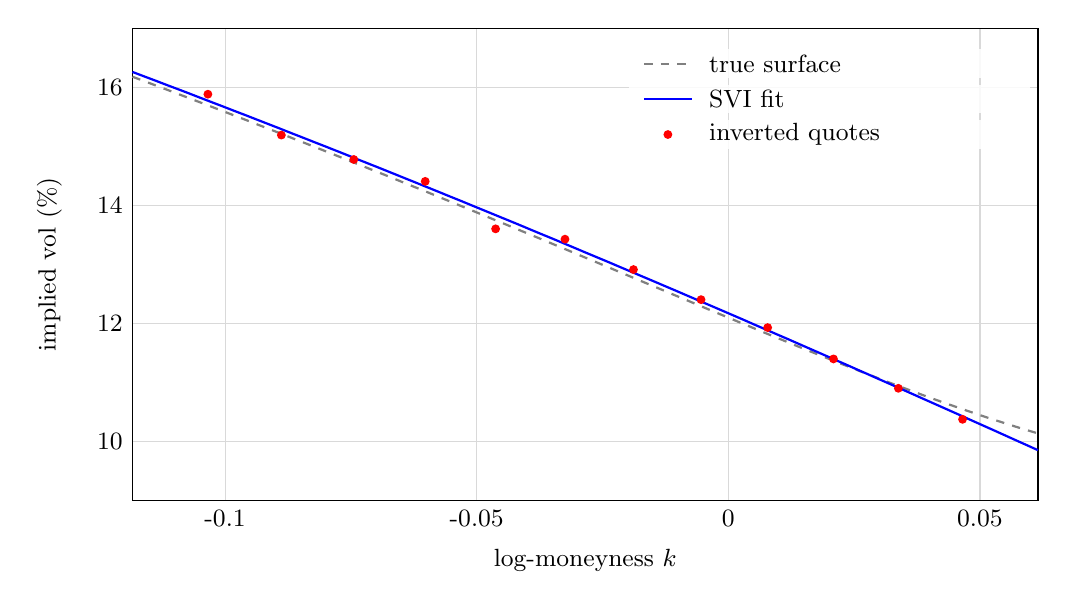
\begin{tikzpicture}[font=\small]
\draw[gray!30] (1.176,0) -- (1.176,6.0);
\node[below] at (1.176,0) {-0.1};
\draw[gray!30] (4.372,0) -- (4.372,6.0);
\node[below] at (4.372,0) {-0.05};
\draw[gray!30] (7.568,0) -- (7.568,6.0);
\node[below] at (7.568,0) {0};
\draw[gray!30] (10.763,0) -- (10.763,6.0);
\node[below] at (10.763,0) {0.05};
\draw[gray!30] (0,0.750) -- (11.5,0.750);
\node[left] at (0,0.750) {10};
\draw[gray!30] (0,2.250) -- (11.5,2.250);
\node[left] at (0,2.250) {12};
\draw[gray!30] (0,3.750) -- (11.5,3.750);
\node[left] at (0,3.750) {14};
\draw[gray!30] (0,5.250) -- (11.5,5.250);
\node[left] at (0,5.250) {16};
\draw (0,0) rectangle (11.5,6.0);
\node[below=14pt] at (5.75,0) {log-moneyness $k$};
\node[rotate=90,above=22pt] at (0,3.0) {implied vol (\%)};
\draw[gray,thick,dashed] plot coordinates {(0.000,5.384) (0.144,5.330) (0.288,5.276) (0.431,5.222) (0.575,5.167) (0.719,5.112) (0.863,5.057) (1.006,5.002) (1.150,4.947) (1.294,4.891) (1.438,4.836) (1.581,4.780) (1.725,4.724) (1.869,4.668) (2.012,4.611) (2.156,4.555) (2.300,4.498) (2.444,4.441) (2.588,4.384) (2.731,4.326) (2.875,4.269) (3.019,4.211) (3.163,4.154) (3.306,4.096) (3.450,4.037) (3.594,3.979) (3.738,3.921) (3.881,3.862) (4.025,3.803) (4.169,3.744) (4.312,3.685) (4.456,3.626) (4.600,3.566) (4.744,3.507) (4.888,3.447) (5.031,3.388) (5.175,3.328) (5.319,3.268) (5.463,3.208) (5.606,3.148) (5.750,3.087) (5.894,3.027) (6.038,2.967) (6.181,2.906) (6.325,2.846) (6.469,2.785) (6.613,2.725) (6.756,2.665) (6.900,2.604) (7.044,2.544) (7.188,2.483) (7.331,2.423) (7.475,2.363) (7.619,2.303) (7.763,2.243) (7.906,2.184) (8.050,2.124) (8.194,2.065) (8.338,2.006) (8.481,1.947) (8.625,1.889) (8.769,1.831) (8.912,1.774) (9.056,1.717) (9.200,1.660) (9.344,1.604) (9.488,1.548) (9.631,1.493) (9.775,1.439) (9.919,1.385) (10.062,1.332) (10.206,1.280) (10.350,1.229) (10.494,1.179) (10.638,1.129) (10.781,1.081) (10.925,1.033) (11.069,0.987) (11.213,0.941) (11.356,0.897) (11.500,0.854)};
\draw[blue,thick] plot coordinates {(0.000,5.445) (0.144,5.390) (0.288,5.336) (0.431,5.281) (0.575,5.227) (0.719,5.172) (0.863,5.116) (1.006,5.061) (1.150,5.006) (1.294,4.950) (1.438,4.895) (1.581,4.839) (1.725,4.783) (1.869,4.727) (2.012,4.670) (2.156,4.614) (2.300,4.557) (2.444,4.501) (2.588,4.444) (2.731,4.387) (2.875,4.329) (3.019,4.272) (3.163,4.215) (3.306,4.157) (3.450,4.099) (3.594,4.041) (3.738,3.983) (3.881,3.925) (4.025,3.866) (4.169,3.808) (4.312,3.749) (4.456,3.690) (4.600,3.631) (4.744,3.572) (4.888,3.513) (5.031,3.453) (5.175,3.393) (5.319,3.334) (5.463,3.274) (5.606,3.214) (5.750,3.153) (5.894,3.093) (6.038,3.033) (6.181,2.972) (6.325,2.911) (6.469,2.850) (6.613,2.789) (6.756,2.728) (6.900,2.667) (7.044,2.605) (7.188,2.543) (7.331,2.482) (7.475,2.420) (7.619,2.358) (7.763,2.296) (7.906,2.233) (8.050,2.171) (8.194,2.108) (8.338,2.046) (8.481,1.983) (8.625,1.920) (8.769,1.857) (8.912,1.794) (9.056,1.731) (9.200,1.667) (9.344,1.604) (9.488,1.540) (9.631,1.477) (9.775,1.413) (9.919,1.349) (10.062,1.285) (10.206,1.221) (10.350,1.157) (10.494,1.093) (10.638,1.028) (10.781,0.964) (10.925,0.900) (11.069,0.835) (11.213,0.770) (11.356,0.706) (11.500,0.641)};
\fill[red] (0.958,5.162) circle (1.6pt);
\fill[red] (1.891,4.643) circle (1.6pt);
\fill[red] (2.811,4.333) circle (1.6pt);
\fill[red] (3.718,4.055) circle (1.6pt);
\fill[red] (4.612,3.452) circle (1.6pt);
\fill[red] (5.493,3.321) circle (1.6pt);
\fill[red] (6.363,2.935) circle (1.6pt);
\fill[red] (7.221,2.553) circle (1.6pt);
\fill[red] (8.067,2.198) circle (1.6pt);
\fill[red] (8.903,1.800) circle (1.6pt);
\fill[red] (9.727,1.427) circle (1.6pt);
\fill[red] (10.542,1.033) circle (1.6pt);
\fill[white,opacity=0.85] (6.3,5.37) rectangle (11.4,5.7299999999999995);
\draw[gray,thick,dashed] (6.5,5.55) -- (7.1,5.55);
\node[right] at (7.2,5.55) {true surface};
\fill[white,opacity=0.85] (6.3,4.92) rectangle (11.4,5.279999999999999);
\draw[blue,thick] (6.5,5.1) -- (7.1,5.1);
\node[right] at (7.2,5.1) {SVI fit};
\fill[white,opacity=0.85] (6.3,4.47) rectangle (11.4,4.829999999999999);
\fill[red] (6.8,4.6499999999999995) circle (1.6pt);
\node[right] at (7.2,4.6499999999999995) {inverted quotes};
\end{tikzpicture}

\caption{The 21 March smile. The inverted quotes (dots) are noisy at the level of
a hundredth of a vol point; the SVI fit (blue) is indistinguishable from the true
surface (dashed gray) on the quoted range.}
\end{figure}

\begin{center}
\begin{minipage}{0.48\textwidth}
\begin{center}\small
\begin{tabular}{|l|r|}
\hline
quantity & value \\ \hline
$a$ & -0.00224 \\
$b$ & 0.01500 \\
$\rho$ & -0.7126 \\
$m$ & 0.1447 \\
$s$ & 0.2124 \\
quotes used & 12 \\
RMSE (vol points) & 0.091 \\
$\min g(k)$ & 0.573 \\
$a+bs\sqrt{1-\rho^2}$ & 0.00000 \\
\hline
\end{tabular}
\end{center}

\end{minipage}
\end{center}

The fitted minimum variance $a+bs\sqrt{1-\rho^2}$ is zero to rounding: the
constraint is \emph{active}, i.e.\ the optimizer pushed the vertex to the
boundary of the admissible region. The butterfly function stays positive
($\min g=\mathbf{0.57}$ on the grid), so the density is non-negative.

\subsection{Across all expiries}

\begin{center}\footnotesize
\begin{tabular}{|l|r|r|r|r|r|r|r|r|r|}
\hline
expiry & days & $F$ & $r$ \% & $q$ \% & n & ATM fit & ATM true & err. & max bias \\ \hline
2025-02-21 & 50 & 37.614 & 3.173 & 4.85 & 8 & 11.95 & 11.91 & 0.04 & 1.94 \\
2025-03-21 & 78 & 37.704 & 3.156 & 3.11 & 12 & 12.17 & 12.10 & 0.07 & 0.31 \\
2025-04-17 & 105 & 37.785 & 3.135 & 2.36 & 15 & 12.20 & 12.26 & $-$0.06 & 0.36 \\
2025-05-16 & 134 & 37.882 & 3.110 & 1.80 & 17 & 12.42 & 12.42 & 0.00 & 0.42 \\
2025-06-20 & 169 & 37.729 & 3.078 & 2.91 & 19 & 12.60 & 12.58 & 0.02 & 0.37 \\
2025-07-18 & 197 & 37.803 & 3.060 & 2.55 & 21 & 12.71 & 12.69 & 0.02 & 0.41 \\
2025-08-15 & 225 & 37.904 & 3.047 & 2.17 & 22 & 12.77 & 12.78 & $-$0.02 & 0.51 \\
2025-09-19 & 260 & 37.729 & 3.032 & 2.93 & 24 & 12.85 & 12.89 & $-$0.04 & 0.47 \\
2025-10-17 & 288 & 37.818 & 3.019 & 2.62 & 24 & 12.98 & 12.96 & 0.02 & 0.37 \\
2025-11-21 & 323 & 37.572 & 3.004 & 3.39 & 26 & 13.02 & 13.04 & $-$0.02 & 1.00 \\
2025-12-19 & 351 & 37.673 & 2.991 & 3.07 & 26 & 13.11 & 13.10 & 0.01 & 0.50 \\
2026-01-16 & 379 & 37.791 & 2.982 & 2.75 & 26 & 13.13 & 13.15 & $-$0.02 & 0.38 \\
\hline
\end{tabular}
\end{center}


(Column key: $F$ forward, $r$ and $q$ the zero rate and implied dividend yield in
percent, $n$ the number of quotes used, ``max bias'' the largest early-exercise
vol bias of the slice in vol points.) Two things stand out. The 21 February
and 21 November expiries have large biases (up to 1.9 and 1.0 points): both fall
on or next to an ex-dividend date, where a call is worth exercising. The 17
January expiry (15 days) is absent: it has only three usable quotes and is
reported as rejected.

\begin{figure}[ht]
\centering
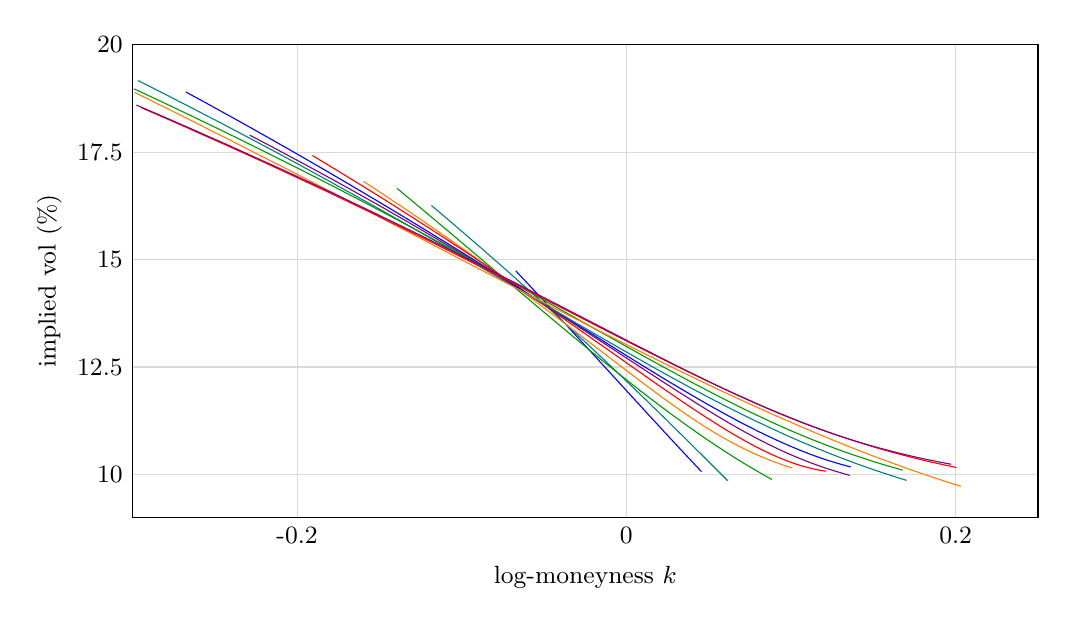
\begin{tikzpicture}[font=\small]
\draw[gray!30] (2.091,0) -- (2.091,6.0);
\node[below] at (2.091,0) {-0.2};
\draw[gray!30] (6.273,0) -- (6.273,6.0);
\node[below] at (6.273,0) {0};
\draw[gray!30] (10.455,0) -- (10.455,6.0);
\node[below] at (10.455,0) {0.2};
\draw[gray!30] (0,0.545) -- (11.5,0.545);
\node[left] at (0,0.545) {10};
\draw[gray!30] (0,1.909) -- (11.5,1.909);
\node[left] at (0,1.909) {12.5};
\draw[gray!30] (0,3.273) -- (11.5,3.273);
\node[left] at (0,3.273) {15};
\draw[gray!30] (0,4.636) -- (11.5,4.636);
\node[left] at (0,4.636) {17.5};
\draw[gray!30] (0,6.000) -- (11.5,6.000);
\node[left] at (0,6.000) {20};
\draw (0,0) rectangle (11.5,6.0);
\node[below=14pt] at (5.75,0) {log-moneyness $k$};
\node[rotate=90,above=22pt] at (0,3.0) {implied vol (\%)};
\draw[blue,thin] plot coordinates {(4.867,3.131) (4.896,3.100) (4.926,3.069) (4.955,3.037) (4.985,3.006) (5.014,2.975) (5.044,2.943) (5.073,2.912) (5.103,2.880) (5.132,2.849) (5.162,2.817) (5.191,2.785) (5.221,2.754) (5.250,2.722) (5.280,2.690) (5.309,2.659) (5.339,2.627) (5.368,2.595) (5.398,2.563) (5.427,2.531) (5.457,2.499) (5.486,2.468) (5.516,2.436) (5.545,2.404) (5.575,2.372) (5.604,2.340) (5.634,2.308) (5.663,2.276) (5.693,2.244) (5.722,2.211) (5.752,2.179) (5.781,2.147) (5.811,2.115) (5.840,2.083) (5.870,2.051) (5.899,2.019) (5.928,1.986) (5.958,1.954) (5.987,1.922) (6.017,1.890) (6.046,1.858) (6.076,1.825) (6.105,1.793) (6.135,1.761) (6.164,1.729) (6.194,1.696) (6.223,1.664) (6.253,1.632) (6.282,1.600) (6.312,1.567) (6.341,1.535) (6.371,1.503) (6.400,1.471) (6.430,1.439) (6.459,1.406) (6.489,1.374) (6.518,1.342) (6.548,1.310) (6.577,1.278) (6.607,1.246) (6.636,1.214) (6.666,1.182) (6.695,1.150) (6.725,1.118) (6.754,1.086) (6.784,1.054) (6.813,1.022) (6.843,0.990) (6.872,0.958) (6.902,0.927) (6.931,0.895) (6.961,0.863) (6.990,0.832) (7.020,0.800) (7.049,0.769) (7.079,0.737) (7.108,0.706) (7.138,0.674) (7.167,0.643) (7.197,0.612) (7.226,0.581)};
\draw[teal,thin] plot coordinates {(3.797,3.960) (3.844,3.920) (3.891,3.881) (3.938,3.841) (3.985,3.801) (4.032,3.761) (4.079,3.721) (4.126,3.681) (4.173,3.641) (4.220,3.600) (4.267,3.560) (4.314,3.519) (4.361,3.478) (4.408,3.438) (4.455,3.397) (4.502,3.356) (4.549,3.314) (4.596,3.273) (4.644,3.232) (4.691,3.190) (4.738,3.149) (4.785,3.107) (4.832,3.065) (4.879,3.023) (4.926,2.981) (4.973,2.939) (5.020,2.897) (5.067,2.854) (5.114,2.812) (5.161,2.769) (5.208,2.727) (5.255,2.684) (5.302,2.641) (5.349,2.598) (5.396,2.555) (5.443,2.511) (5.490,2.468) (5.537,2.425) (5.584,2.381) (5.631,2.337) (5.678,2.293) (5.725,2.250) (5.772,2.206) (5.819,2.161) (5.866,2.117) (5.913,2.073) (5.960,2.028) (6.007,1.984) (6.054,1.939) (6.101,1.895) (6.148,1.850) (6.195,1.805) (6.242,1.760) (6.289,1.715) (6.336,1.670) (6.384,1.624) (6.431,1.579) (6.478,1.533) (6.525,1.488) (6.572,1.442) (6.619,1.396) (6.666,1.351) (6.713,1.305) (6.760,1.259) (6.807,1.213) (6.854,1.166) (6.901,1.120) (6.948,1.074) (6.995,1.028) (7.042,0.981) (7.089,0.935) (7.136,0.888) (7.183,0.841) (7.230,0.795) (7.277,0.748) (7.324,0.701) (7.371,0.654) (7.418,0.607) (7.465,0.560) (7.512,0.513) (7.559,0.466)};
\draw[green!60!black,thin] plot coordinates {(3.359,4.179) (3.419,4.129) (3.478,4.080) (3.538,4.030) (3.597,3.980) (3.657,3.931) (3.716,3.881) (3.776,3.831) (3.836,3.781) (3.895,3.731) (3.955,3.681) (4.014,3.631) (4.074,3.581) (4.133,3.530) (4.193,3.480) (4.252,3.430) (4.312,3.379) (4.371,3.329) (4.431,3.279) (4.490,3.228) (4.550,3.178) (4.609,3.127) (4.669,3.077) (4.728,3.026) (4.788,2.976) (4.847,2.926) (4.907,2.875) (4.966,2.825) (5.026,2.775) (5.085,2.724) (5.145,2.674) (5.204,2.624) (5.264,2.574) (5.323,2.524) (5.383,2.474) (5.442,2.425) (5.502,2.375) (5.561,2.325) (5.621,2.276) (5.680,2.227) (5.740,2.178) (5.799,2.129) (5.859,2.080) (5.919,2.031) (5.978,1.983) (6.038,1.935) (6.097,1.887) (6.157,1.839) (6.216,1.792) (6.276,1.745) (6.335,1.698) (6.395,1.651) (6.454,1.605) (6.514,1.559) (6.573,1.513) (6.633,1.468) (6.692,1.423) (6.752,1.378) (6.811,1.334) (6.871,1.290) (6.930,1.247) (6.990,1.204) (7.049,1.161) (7.109,1.119) (7.168,1.077) (7.228,1.036) (7.287,0.995) (7.347,0.955) (7.406,0.915) (7.466,0.876) (7.525,0.837) (7.585,0.799) (7.644,0.761) (7.704,0.724) (7.763,0.688) (7.823,0.652) (7.882,0.617) (7.942,0.582) (8.002,0.548) (8.061,0.514) (8.121,0.481)};
\draw[orange,thin] plot coordinates {(2.934,4.267) (3.002,4.222) (3.070,4.178) (3.138,4.133) (3.206,4.088) (3.274,4.043) (3.343,3.997) (3.411,3.952) (3.479,3.906) (3.547,3.860) (3.615,3.814) (3.683,3.768) (3.751,3.721) (3.819,3.674) (3.887,3.627) (3.955,3.580) (4.023,3.533) (4.091,3.485) (4.159,3.437) (4.228,3.389) (4.296,3.341) (4.364,3.292) (4.432,3.244) (4.500,3.195) (4.568,3.146) (4.636,3.097) (4.704,3.047) (4.772,2.997) (4.840,2.947) (4.908,2.897) (4.976,2.847) (5.045,2.797) (5.113,2.746) (5.181,2.695) (5.249,2.644) (5.317,2.593) (5.385,2.542) (5.453,2.490) (5.521,2.439) (5.589,2.387) (5.657,2.335) (5.725,2.283) (5.793,2.231) (5.861,2.179) (5.930,2.127) (5.998,2.075) (6.066,2.023) (6.134,1.971) (6.202,1.919) (6.270,1.867) (6.338,1.815) (6.406,1.764) (6.474,1.712) (6.542,1.661) (6.610,1.611) (6.678,1.560) (6.746,1.511) (6.815,1.461) (6.883,1.413) (6.951,1.365) (7.019,1.318) (7.087,1.271) (7.155,1.226) (7.223,1.181) (7.291,1.138) (7.359,1.096) (7.427,1.055) (7.495,1.015) (7.563,0.977) (7.632,0.940) (7.700,0.904) (7.768,0.870) (7.836,0.837) (7.904,0.806) (7.972,0.776) (8.040,0.748) (8.108,0.721) (8.176,0.696) (8.244,0.671) (8.312,0.648) (8.380,0.627)};
\draw[red,thin] plot coordinates {(2.286,4.595) (2.367,4.546) (2.449,4.497) (2.530,4.447) (2.612,4.398) (2.693,4.348) (2.775,4.298) (2.856,4.248) (2.938,4.198) (3.020,4.147) (3.101,4.097) (3.183,4.046) (3.264,3.994) (3.346,3.943) (3.427,3.891) (3.509,3.839) (3.590,3.787) (3.672,3.735) (3.753,3.683) (3.835,3.630) (3.916,3.577) (3.998,3.524) (4.079,3.470) (4.161,3.417) (4.242,3.363) (4.324,3.309) (4.406,3.254) (4.487,3.200) (4.569,3.145) (4.650,3.090) (4.732,3.035) (4.813,2.980) (4.895,2.924) (4.976,2.868) (5.058,2.812) (5.139,2.756) (5.221,2.700) (5.302,2.644) (5.384,2.587) (5.465,2.530) (5.547,2.473) (5.629,2.416) (5.710,2.359) (5.792,2.302) (5.873,2.244) (5.955,2.187) (6.036,2.130) (6.118,2.072) (6.199,2.015) (6.281,1.957) (6.362,1.900) (6.444,1.843) (6.525,1.786) (6.607,1.729) (6.688,1.672) (6.770,1.616) (6.852,1.560) (6.933,1.504) (7.015,1.449) (7.096,1.394) (7.178,1.340) (7.259,1.287) (7.341,1.235) (7.422,1.183) (7.504,1.133) (7.585,1.083) (7.667,1.035) (7.748,0.989) (7.830,0.943) (7.911,0.900) (7.993,0.859) (8.075,0.819) (8.156,0.782) (8.238,0.747) (8.319,0.715) (8.401,0.685) (8.482,0.659) (8.564,0.636) (8.645,0.616) (8.727,0.599) (8.808,0.586)};
\draw[violet,thin] plot coordinates {(1.489,4.854) (1.585,4.804) (1.680,4.754) (1.775,4.704) (1.870,4.653) (1.966,4.602) (2.061,4.551) (2.156,4.500) (2.251,4.449) (2.347,4.397) (2.442,4.345) (2.537,4.293) (2.632,4.240) (2.728,4.188) (2.823,4.135) (2.918,4.081) (3.013,4.028) (3.109,3.974) (3.204,3.920) (3.299,3.865) (3.394,3.811) (3.490,3.756) (3.585,3.700) (3.680,3.645) (3.775,3.589) (3.871,3.533) (3.966,3.476) (4.061,3.420) (4.156,3.363) (4.252,3.305) (4.347,3.248) (4.442,3.190) (4.537,3.131) (4.633,3.073) (4.728,3.014) (4.823,2.955) (4.918,2.895) (5.013,2.836) (5.109,2.776) (5.204,2.716) (5.299,2.655) (5.394,2.594) (5.490,2.533) (5.585,2.472) (5.680,2.410) (5.775,2.349) (5.871,2.287) (5.966,2.225) (6.061,2.163) (6.156,2.101) (6.252,2.038) (6.347,1.976) (6.442,1.914) (6.537,1.851) (6.633,1.789) (6.728,1.727) (6.823,1.666) (6.918,1.604) (7.014,1.544) (7.109,1.483) (7.204,1.423) (7.299,1.365) (7.395,1.306) (7.490,1.249) (7.585,1.193) (7.680,1.139) (7.776,1.085) (7.871,1.034) (7.966,0.984) (8.061,0.935) (8.157,0.889) (8.252,0.844) (8.347,0.801) (8.442,0.761) (8.538,0.722) (8.633,0.686) (8.728,0.651) (8.823,0.619) (8.919,0.589) (9.014,0.560) (9.109,0.533)};
\draw[blue,thin] plot coordinates {(0.680,5.401) (0.785,5.344) (0.891,5.286) (0.996,5.229) (1.102,5.170) (1.207,5.112) (1.313,5.054) (1.418,4.995) (1.524,4.936) (1.629,4.876) (1.735,4.817) (1.840,4.757) (1.946,4.697) (2.052,4.637) (2.157,4.576) (2.263,4.515) (2.368,4.454) (2.474,4.393) (2.579,4.331) (2.685,4.269) (2.790,4.207) (2.896,4.145) (3.001,4.082) (3.107,4.020) (3.212,3.957) (3.318,3.893) (3.423,3.830) (3.529,3.766) (3.634,3.702) (3.740,3.638) (3.846,3.573) (3.951,3.509) (4.057,3.444) (4.162,3.379) (4.268,3.313) (4.373,3.248) (4.479,3.182) (4.584,3.117) (4.690,3.051) (4.795,2.984) (4.901,2.918) (5.006,2.852) (5.112,2.785) (5.217,2.719) (5.323,2.652) (5.428,2.586) (5.534,2.519) (5.640,2.453) (5.745,2.386) (5.851,2.320) (5.956,2.253) (6.062,2.187) (6.167,2.121) (6.273,2.055) (6.378,1.990) (6.484,1.924) (6.589,1.860) (6.695,1.795) (6.800,1.731) (6.906,1.668) (7.011,1.606) (7.117,1.544) (7.222,1.483) (7.328,1.422) (7.434,1.363) (7.539,1.305) (7.645,1.248) (7.750,1.192) (7.856,1.138) (7.961,1.085) (8.067,1.034) (8.172,0.985) (8.278,0.937) (8.383,0.892) (8.489,0.848) (8.594,0.807) (8.700,0.768) (8.805,0.732) (8.911,0.699) (9.017,0.668) (9.122,0.640)};
\draw[teal,thin] plot coordinates {(0.071,5.547) (0.195,5.485) (0.318,5.422) (0.442,5.360) (0.565,5.296) (0.689,5.233) (0.812,5.169) (0.936,5.105) (1.059,5.041) (1.183,4.977) (1.306,4.912) (1.430,4.846) (1.553,4.781) (1.677,4.715) (1.801,4.649) (1.924,4.583) (2.048,4.516) (2.171,4.449) (2.295,4.381) (2.418,4.314) (2.542,4.246) (2.665,4.177) (2.789,4.109) (2.912,4.040) (3.036,3.971) (3.160,3.902) (3.283,3.832) (3.407,3.762) (3.530,3.692) (3.654,3.621) (3.777,3.550) (3.901,3.479) (4.024,3.408) (4.148,3.337) (4.271,3.265) (4.395,3.193) (4.519,3.122) (4.642,3.050) (4.766,2.977) (4.889,2.905) (5.013,2.833) (5.136,2.760) (5.260,2.688) (5.383,2.616) (5.507,2.544) (5.630,2.471) (5.754,2.399) (5.877,2.328) (6.001,2.256) (6.125,2.185) (6.248,2.114) (6.372,2.044) (6.495,1.974) (6.619,1.904) (6.742,1.835) (6.866,1.767) (6.989,1.700) (7.113,1.633) (7.236,1.567) (7.360,1.502) (7.484,1.438) (7.607,1.375) (7.731,1.314) (7.854,1.253) (7.978,1.194) (8.101,1.136) (8.225,1.079) (8.348,1.023) (8.472,0.969) (8.595,0.917) (8.719,0.866) (8.843,0.816) (8.966,0.768) (9.090,0.721) (9.213,0.675) (9.337,0.631) (9.460,0.589) (9.584,0.548) (9.707,0.508) (9.831,0.470)};
\draw[green!60!black,thin] plot coordinates {(0.022,5.441) (0.145,5.384) (0.269,5.326) (0.392,5.268) (0.516,5.209) (0.639,5.151) (0.763,5.092) (0.886,5.032) (1.010,4.973) (1.133,4.913) (1.257,4.853) (1.381,4.792) (1.504,4.731) (1.628,4.670) (1.751,4.609) (1.875,4.547) (1.998,4.485) (2.122,4.423) (2.245,4.360) (2.369,4.297) (2.492,4.234) (2.616,4.170) (2.739,4.106) (2.863,4.042) (2.987,3.978) (3.110,3.913) (3.234,3.848) (3.357,3.782) (3.481,3.716) (3.604,3.650) (3.728,3.584) (3.851,3.517) (3.975,3.450) (4.098,3.383) (4.222,3.316) (4.346,3.248) (4.469,3.180) (4.593,3.111) (4.716,3.043) (4.840,2.974) (4.963,2.905) (5.087,2.836) (5.210,2.767) (5.334,2.697) (5.457,2.628) (5.581,2.558) (5.704,2.489) (5.828,2.419) (5.952,2.350) (6.075,2.281) (6.199,2.211) (6.322,2.142) (6.446,2.074) (6.569,2.005) (6.693,1.937) (6.816,1.870) (6.940,1.803) (7.063,1.736) (7.187,1.671) (7.311,1.606) (7.434,1.542) (7.558,1.479) (7.681,1.418) (7.805,1.357) (7.928,1.298) (8.052,1.240) (8.175,1.183) (8.299,1.128) (8.422,1.075) (8.546,1.023) (8.670,0.973) (8.793,0.925) (8.917,0.878) (9.040,0.833) (9.164,0.790) (9.287,0.749) (9.411,0.709) (9.534,0.671) (9.658,0.635) (9.781,0.600)};
\draw[orange,thin] plot coordinates {(0.030,5.396) (0.172,5.326) (0.313,5.255) (0.455,5.185) (0.597,5.114) (0.739,5.043) (0.880,4.972) (1.022,4.900) (1.164,4.829) (1.306,4.757) (1.447,4.685) (1.589,4.612) (1.731,4.540) (1.873,4.468) (2.015,4.395) (2.156,4.322) (2.298,4.249) (2.440,4.176) (2.582,4.103) (2.723,4.029) (2.865,3.956) (3.007,3.882) (3.149,3.808) (3.290,3.735) (3.432,3.661) (3.574,3.587) (3.716,3.513) (3.857,3.439) (3.999,3.365) (4.141,3.291) (4.283,3.217) (4.424,3.143) (4.566,3.070) (4.708,2.996) (4.850,2.922) (4.991,2.849) (5.133,2.775) (5.275,2.702) (5.417,2.629) (5.559,2.556) (5.700,2.484) (5.842,2.412) (5.984,2.340) (6.126,2.268) (6.267,2.197) (6.409,2.126) (6.551,2.055) (6.693,1.985) (6.834,1.916) (6.976,1.847) (7.118,1.778) (7.260,1.710) (7.401,1.643) (7.543,1.576) (7.685,1.511) (7.827,1.445) (7.968,1.381) (8.110,1.317) (8.252,1.255) (8.394,1.193) (8.535,1.132) (8.677,1.072) (8.819,1.013) (8.961,0.955) (9.102,0.898) (9.244,0.842) (9.386,0.787) (9.528,0.734) (9.670,0.682) (9.811,0.630) (9.953,0.581) (10.095,0.532) (10.237,0.485) (10.378,0.439) (10.520,0.394)};
\draw[red,thin] plot coordinates {(0.116,5.201) (0.257,5.140) (0.399,5.078) (0.541,5.016) (0.683,4.953) (0.824,4.890) (0.966,4.827) (1.108,4.764) (1.250,4.700) (1.392,4.636) (1.533,4.572) (1.675,4.507) (1.817,4.442) (1.959,4.376) (2.100,4.310) (2.242,4.244) (2.384,4.178) (2.526,4.111) (2.667,4.044) (2.809,3.976) (2.951,3.908) (3.093,3.840) (3.234,3.771) (3.376,3.702) (3.518,3.633) (3.660,3.563) (3.801,3.494) (3.943,3.423) (4.085,3.353) (4.227,3.282) (4.368,3.211) (4.510,3.139) (4.652,3.068) (4.794,2.996) (4.936,2.924) (5.077,2.852) (5.219,2.779) (5.361,2.707) (5.503,2.634) (5.644,2.562) (5.786,2.489) (5.928,2.417) (6.070,2.344) (6.211,2.272) (6.353,2.200) (6.495,2.128) (6.637,2.057) (6.778,1.987) (6.920,1.917) (7.062,1.847) (7.204,1.779) (7.345,1.711) (7.487,1.644) (7.629,1.579) (7.771,1.515) (7.912,1.452) (8.054,1.390) (8.196,1.331) (8.338,1.273) (8.479,1.216) (8.621,1.162) (8.763,1.110) (8.905,1.059) (9.047,1.011) (9.188,0.964) (9.330,0.920) (9.472,0.877) (9.614,0.837) (9.755,0.799) (9.897,0.762) (10.039,0.727) (10.181,0.694) (10.322,0.663) (10.464,0.633)};
\draw[violet,thin] plot coordinates {(0.050,5.236) (0.192,5.175) (0.333,5.114) (0.475,5.053) (0.617,4.991) (0.759,4.929) (0.900,4.866) (1.042,4.804) (1.184,4.741) (1.326,4.677) (1.467,4.613) (1.609,4.549) (1.751,4.485) (1.893,4.420) (2.035,4.355) (2.176,4.289) (2.318,4.223) (2.460,4.157) (2.602,4.090) (2.743,4.023) (2.885,3.955) (3.027,3.888) (3.169,3.819) (3.310,3.751) (3.452,3.682) (3.594,3.613) (3.736,3.543) (3.877,3.473) (4.019,3.403) (4.161,3.332) (4.303,3.261) (4.444,3.190) (4.586,3.118) (4.728,3.046) (4.870,2.974) (5.011,2.901) (5.153,2.828) (5.295,2.755) (5.437,2.682) (5.578,2.609) (5.720,2.536) (5.862,2.463) (6.004,2.389) (6.146,2.316) (6.287,2.243) (6.429,2.170) (6.571,2.098) (6.713,2.026) (6.854,1.954) (6.996,1.883) (7.138,1.813) (7.280,1.744) (7.421,1.675) (7.563,1.608) (7.705,1.543) (7.847,1.478) (7.988,1.416) (8.130,1.355) (8.272,1.296) (8.414,1.239) (8.555,1.184) (8.697,1.131) (8.839,1.081) (8.981,1.033) (9.122,0.987) (9.264,0.944) (9.406,0.903) (9.548,0.864) (9.690,0.827) (9.831,0.793) (9.973,0.760) (10.115,0.730) (10.257,0.701) (10.398,0.674)};
\end{tikzpicture}

\caption{All twelve fitted smiles. Short expiries are steeper and the skew
flattens with maturity. The calendar condition $\partial_Tw\ge0$, which the code
checks on total variance over the common strike range, holds.}
\end{figure}

\begin{figure}[ht]
\centering
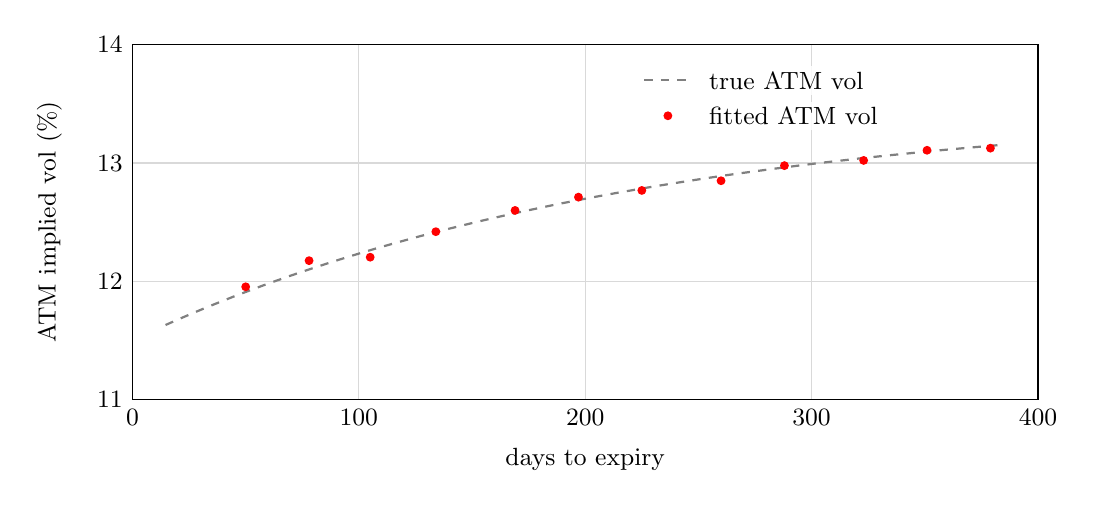
\begin{tikzpicture}[font=\small]
\draw[gray!30] (0.000,0) -- (0.000,4.5);
\node[below] at (0.000,0) {0};
\draw[gray!30] (2.875,0) -- (2.875,4.5);
\node[below] at (2.875,0) {100};
\draw[gray!30] (5.750,0) -- (5.750,4.5);
\node[below] at (5.750,0) {200};
\draw[gray!30] (8.625,0) -- (8.625,4.5);
\node[below] at (8.625,0) {300};
\draw[gray!30] (11.500,0) -- (11.500,4.5);
\node[below] at (11.500,0) {400};
\draw[gray!30] (0,0.000) -- (11.5,0.000);
\node[left] at (0,0.000) {11};
\draw[gray!30] (0,1.500) -- (11.5,1.500);
\node[left] at (0,1.500) {12};
\draw[gray!30] (0,3.000) -- (11.5,3.000);
\node[left] at (0,3.000) {13};
\draw[gray!30] (0,4.500) -- (11.5,4.500);
\node[left] at (0,4.500) {14};
\draw (0,0) rectangle (11.5,4.5);
\node[below=14pt] at (5.75,0) {days to expiry};
\node[rotate=90,above=22pt] at (0,2.25) {ATM implied vol (\%)};
\draw[gray,thick,dashed] plot coordinates {(0.420,0.943) (0.599,1.022) (0.779,1.099) (0.959,1.174) (1.138,1.246) (1.318,1.317) (1.498,1.385) (1.677,1.452) (1.857,1.516) (2.036,1.579) (2.216,1.640) (2.396,1.699) (2.575,1.757) (2.755,1.813) (2.935,1.868) (3.114,1.921) (3.294,1.972) (3.474,2.022) (3.653,2.071) (3.833,2.118) (4.013,2.164) (4.192,2.208) (4.372,2.252) (4.551,2.294) (4.731,2.335) (4.911,2.375) (5.090,2.413) (5.270,2.451) (5.450,2.488) (5.629,2.523) (5.809,2.558) (5.989,2.591) (6.168,2.624) (6.348,2.655) (6.527,2.686) (6.707,2.716) (6.887,2.745) (7.066,2.773) (7.246,2.801) (7.426,2.828) (7.605,2.854) (7.785,2.879) (7.965,2.903) (8.144,2.927) (8.324,2.950) (8.503,2.973) (8.683,2.995) (8.863,3.016) (9.042,3.036) (9.222,3.057) (9.402,3.076) (9.581,3.095) (9.761,3.113) (9.941,3.131) (10.120,3.149) (10.300,3.166) (10.480,3.182) (10.659,3.198) (10.839,3.214) (11.018,3.229)};
\fill[red] (1.438,1.428) circle (1.6pt);
\fill[red] (2.243,1.760) circle (1.6pt);
\fill[red] (3.019,1.804) circle (1.6pt);
\fill[red] (3.853,2.128) circle (1.6pt);
\fill[red] (4.859,2.398) circle (1.6pt);
\fill[red] (5.664,2.567) circle (1.6pt);
\fill[red] (6.469,2.652) circle (1.6pt);
\fill[red] (7.475,2.775) circle (1.6pt);
\fill[red] (8.280,2.967) circle (1.6pt);
\fill[red] (9.286,3.033) circle (1.6pt);
\fill[red] (10.091,3.162) circle (1.6pt);
\fill[red] (10.896,3.189) circle (1.6pt);
\fill[white,opacity=0.85] (6.3,3.8699999999999997) rectangle (11.4,4.2299999999999995);
\draw[gray,thick,dashed] (6.5,4.05) -- (7.1,4.05);
\node[right] at (7.2,4.05) {true ATM vol};
\fill[white,opacity=0.85] (6.3,3.4199999999999995) rectangle (11.4,3.78);
\fill[red] (6.8,3.5999999999999996) circle (1.6pt);
\node[right] at (7.2,3.5999999999999996) {fitted ATM vol};
\end{tikzpicture}

\caption{ATM volatility term structure: fitted values (dots) against the true
curve (dashed).}
\end{figure}

\subsection{The same steps in Python}\label{sec:python}

Everything above can be reproduced from a Python session. The snippets are run by
\texttt{docs/\allowbreak build\_\allowbreak walkthrough.py}, and the output shown is what the code printed,
so it cannot drift from the library.

\paragraph{The chain.}
{\footnotesize
\begin{verbatim}
from tsx60_iv.synthetic import generate_realistic_chain
chain = generate_realistic_chain()
print(chain.shape)
cols = ["expiration", "option_type", "strike", "bid", "ask", "volume"]
print(chain[cols].head(4).to_string(index=False))
\end{verbatim}
\vspace{-0.6em}
\begin{verbatim}
(780, 11)
expiration option_type  strike  bid   ask  volume
2025-01-17        call    28.0 9.57 10.07     0.0
2025-01-17        call    29.0 8.61  9.05     0.0
2025-01-17        call    30.0 7.63  8.03     0.0
2025-01-17        call    31.0 6.53  6.88     0.0
\end{verbatim}
}

\paragraph{One expiry, calls and puts side by side.}
{\footnotesize
\begin{verbatim}
e = chain[chain.expiration == "2025-03-21"]
window = e[e.strike.between(36, 39)]
print(window.pivot(index="strike", columns="option_type",
                   values=["bid", "ask"]).to_string())
\end{verbatim}
\vspace{-0.6em}
\begin{verbatim}
              bid         ask      
option_type  call   put  call   put
strike                             
36.0         2.03  0.30  2.14  0.33
36.5         1.63  0.43  1.73  0.46
37.0         1.28  0.57  1.36  0.61
37.5         0.95  0.75  1.01  0.80
38.0         0.69  0.96  0.73  1.02
38.5         0.46  1.24  0.49  1.32
39.0         0.28  1.57  0.31  1.66
\end{verbatim}
}

\paragraph{Quality filter, time to expiry, rate and discount.}
{\footnotesize
\begin{verbatim}
from tsx60_iv.rates import RateCurve
from tsx60_iv.synthetic import BOC_CURVE_PATH
from tsx60_iv.data import estimate_forward_and_rates

curve = RateCurve.from_json(BOC_CURVE_PATH)
spot = float(chain.spot.iloc[0])
clean = estimate_forward_and_rates(chain, spot, curve)
c = clean[clean.expiration == "2025-03-21"]
print(len(e), "quotes,", len(c), "pass the quality filter")
cols = ["strike", "option_type", "mid", "time_to_expiry", "rate", "discount"]
print(c[cols].head(3).to_string(index=False))
\end{verbatim}
\vspace{-0.6em}
\begin{verbatim}
60 quotes, 42 pass the quality filter
 strike option_type   mid  time_to_expiry     rate  discount
   28.0        call 9.840        0.213699 0.031559  0.993279
   29.0        call 8.750        0.213699 0.031559  0.993279
   30.0        call 7.875        0.213699 0.031559  0.993279
\end{verbatim}
}

\paragraph{Put-call parity by hand: the forward from the three at-the-money pairs.}
{\footnotesize
\begin{verbatim}
D = c.discount.iloc[0]
pairs = c.pivot(index="strike", columns="option_type", values="mid").dropna()
K = pairs.index.to_numpy()
pairs["F_hat"] = K + (pairs.call - pairs.put) / D
near = pairs.iloc[np.argsort(np.abs(K - spot))[:3]]
print(near.round(4).to_string())
print("median F =", round(near.F_hat.median(), 4))
\end{verbatim}
\vspace{-0.6em}
\begin{verbatim}
option_type  call    put    F_hat
strike                           
37.5         0.98  0.775  37.7064
38.0         0.71  0.990  37.7181
37.0         1.32  0.590  37.7349
median F = 37.7181
\end{verbatim}
}

\paragraph{Correcting the forward for early exercise (three passes).}
{\footnotesize
\begin{verbatim}
from tsx60_iv.bsm import implied_volatility
from tsx60_iv.american import early_exercise_bias
from tsx60_iv.market_params import expected_dividends, load_params
from tsx60_iv.synthetic import MARKET_PARAMS_PATH

dividends = expected_dividends(load_params(MARKET_PARAMS_PATH))
T, r = c.time_to_expiry.iloc[0], c.rate.iloc[0]
Kn = near.index.to_numpy()
F = near.F_hat.median()
for step in range(3):
    adjusted = {}
    for side in ("call", "put"):
        iv = [implied_volatility(m, F, k, T, D, side)
              for k, m in zip(Kn, near[side])]
        premium, _ = early_exercise_bias(np.array(iv), spot, F, Kn, T, r, side,
                                         dividends=dividends)
        adjusted[side] = near[side].to_numpy() - premium
    F = np.median(Kn + (adjusted["call"] - adjusted["put"]) / D)
    print("pass", step + 1, "F =", round(float(F), 4))
\end{verbatim}
\vspace{-0.6em}
\begin{verbatim}
pass 1 F = 37.7084
pass 2 F = 37.7052
pass 3 F = 37.7041
\end{verbatim}
}

\paragraph{Out-of-the-money quotes inverted two ways.}
{\footnotesize
\begin{verbatim}
from tsx60_iv.american import american_implied_vols
otm = c[((c.option_type == "put") & (c.strike < F))
        | ((c.option_type == "call") & (c.strike >= F))]
q = r - np.log(F / spot) / T          # yield implied by the forward
parts = []
for side, g in otm.groupby("option_type"):
    iv_a = american_implied_vols(g.mid.to_numpy(), spot, g.strike.to_numpy(),
                                 T, r, q, side, dividends=dividends)
    iv_e = [implied_volatility(m, F, k, T, D, side)
            for m, k in zip(g.mid, g.strike)]
    parts.append(g.assign(iv_european=100 * np.array(iv_e), iv_american=100 * iv_a))
table = pd.concat(parts).sort_values("strike")
cols = ["strike", "option_type", "mid", "iv_european", "iv_american"]
print(table[cols].round(3).to_string(index=False))
\end{verbatim}
\vspace{-0.6em}
\begin{verbatim}
 strike option_type   mid  iv_european  iv_american
   34.0         put 0.095       15.926       15.882
   34.5         put 0.125       15.246       15.191
   35.0         put 0.175       14.841       14.778
   35.5         put 0.245       14.496       14.406
   36.0         put 0.315       13.712       13.603
   36.5         put 0.445       13.573       13.428
   37.0         put 0.590       13.107       12.914
   37.5         put 0.775       12.670       12.405
   38.0        call 0.710       12.244       11.931
   38.5        call 0.475       11.602       11.400
   39.0        call 0.295       11.024       10.903
   39.5        call 0.165       10.442       10.377
\end{verbatim}
}

\paragraph{Fitting one SVI slice and checking the butterfly condition.}
{\footnotesize
\begin{verbatim}
from tsx60_iv.svi import calibrate_svi_slice, durrleman_g
k = np.log(table.strike.to_numpy() / F)
w = (table.iv_american.to_numpy() / 100) ** 2 * T      # total variance
params = calibrate_svi_slice(k, w)
names = ["a", "b", "rho", "m", "sigma"]
print({n: round(float(v), 5) for n, v in zip(names, params)})
grid = np.linspace(k.min() - 0.1, k.max() + 0.1, 200)
print("min g on the grid:", round(float(durrleman_g(grid, *params).min()), 3))
\end{verbatim}
\vspace{-0.6em}
\begin{verbatim}
{'a': -0.00224, 'b': 0.015, 'rho': -0.71255, 'm': 0.14469, 'sigma': 0.21238}
min g on the grid: 0.457
\end{verbatim}
}

\paragraph{The whole pipeline, then the European variant for comparison.}
{\footnotesize
\begin{verbatim}
from tsx60_iv.surface import build_surface
kw = dict(ticker="XIU (synthetic)", source="synthetic_demo", synthetic=True)
amer = build_surface(chain, spot, curve, exercise="american",
                     dividends=dividends, **kw)
euro = build_surface(chain, spot, curve, exercise="european", **kw)
print("fitted:", len(amer["expiries"]), " rejected:",
      [r["expiration"] for r in amer["rejected"]])
print("calendar arbitrage-free:", amer["calendar"]["ok"])
for a, b in list(zip(amer["expiries"], euro["expiries"]))[2:5]:
    atm = lambda s: 100 * (s["atm_w"] / s["T"]) ** 0.5
    print(a["expiration"], "ATM vol  american %.2f  european %.2f"
          % (atm(a), atm(b)))
\end{verbatim}
\vspace{-0.6em}
\begin{verbatim}
fitted: 12  rejected: ['2025-01-17']
calendar arbitrage-free: True
2025-04-17 ATM vol  american 12.20  european 12.37
2025-05-16 ATM vol  american 12.42  european 12.62
2025-06-20 ATM vol  american 12.60  european 12.85
\end{verbatim}
}


\section{Results}\label{sec:results}

Against the known generating surface (12 of 13 expiries fit):

\begin{center}\footnotesize
\begin{tabular}{|l|r|r|r|r|}
\hline
variant & expiries fitted & mean ATM error & worst ATM error & worst quote error \\ \hline
American, schedule (default) & 12 & 0.003 & 0.07 & 0.31 \\
American, continuous yield & 11 & 0.238 & 0.72 & 1.02 \\
European & 12 & 0.274 & 0.73 & 1.05 \\
\hline
\end{tabular}
\end{center}


(All in volatility points.) The pipeline with the American tree and the discrete
dividend schedule recovers the ATM level to well under a tenth of a vol point on
average. Treating the same quotes as European overstates ATM volatility by
\atmErrEuropean\ points on average and up to \atmWorstEuropean, and the worst single
quote is off by \quoteWorstEuropean\ points. A continuous yield improves on
this but not by much (\atmErrContinuous\ points against
\atmErrEuropean): the bias comes mostly from calls just before ex-dividend dates,
which only the discrete schedule values correctly. The forward correction of
Section~\ref{sec:fcorr} is part of the default: without it the forward of the
ex-date expiry is off by 0.33\% and its smile by about one vol point.

\paragraph{What the tests cover.} The BSM Greeks against finite differences; the
tree against closed-form BSM, against a published American put value (about 6.09
for $S=K=100$, $r=5\%$, $\sigma=20\%$, $T=1$), dominance of the American price,
and put-call symmetry; discrete versus continuous dividends; the rate curve
(conversion, bootstrap on flat and sloped curves, stale prints, a mocked single
Valet request); the SSVI conditions and exact raw-SVI form of every slice; the
generated chain (determinism, ticks, spreads, Good Friday); the forward
correction; and the whole pipeline against the generating surface.

% =====================================================================
\part{Limitations and further reading}
% =====================================================================

\section{Limitations and extensions}

\begin{itemize}
  \item \textbf{Synthetic data.} No real quote has been used. Real chains add
        stale quotes, crossed markets and irregular strikes; the pipeline's
        reject-and-report design is aimed at that, but it has not been tested on
        it.
  \item \textbf{Constant-volatility tree.} The American price inside the pipeline
        uses a flat volatility per quote (the usual convention) rather than a
        local-volatility or stochastic-volatility model.
  \item \textbf{Dividends.} The expected schedule is the trailing four, repeated
        with no growth, and dividends are discounted at the expiry's own zero
        rate.
  \item \textbf{Rates.} A single snapshot (2025-01-02), flat beyond two years.
  \item \textbf{Fit.} Local multi-start SLSQP. The grid-based butterfly check
        cannot rule out violations between grid points.
  \item \textbf{Extensions.} Real data through a licensed feed; a calendar
        constraint inside the fit; a discrete-dividend tree with growth; and
        pricing exotics off the calibrated surface.
\end{itemize}

\begin{thebibliography}{99}
\bibitem{bs73} F.~Black and M.~Scholes, The pricing of options and corporate
liabilities, \emph{J. Political Economy} 81 (1973).
\bibitem{b76} F.~Black, The pricing of commodity contracts, \emph{J. Financial
Economics} 3 (1976).
\bibitem{crr79} J.~Cox, S.~Ross and M.~Rubinstein, Option pricing: a simplified
approach, \emph{J. Financial Economics} 7 (1979).
\bibitem{lee04} R.~Lee, The moment formula for implied volatility at extreme
strikes, \emph{Mathematical Finance} 14 (2004).
\bibitem{gat04} J.~Gatheral, A parsimonious arbitrage-free implied volatility
parameterization with application to the valuation of volatility derivatives,
Presentation, 2004.
\bibitem{gj14} J.~Gatheral and A.~Jacquier, Arbitrage-free SVI volatility
surfaces, \emph{Quantitative Finance} 14 (2014).
\bibitem{dur05} P.~Durrleman, From implied to spot volatilities, PhD thesis,
Princeton University, 2004.
\bibitem{hull} J.~Hull, \emph{Options, Futures, and Other Derivatives}, Pearson.
\bibitem{shreve} S.~Shreve, \emph{Stochastic Calculus for Finance II:
Continuous-Time Models}, Springer, 2004.
\end{thebibliography}

\appendix
\section{Symbols}

\begin{center}\small
\begin{tabular}{|l|L{11.5cm}|}
\hline
$S,\ F,\ K,\ T$ & spot, forward, strike, time to expiry (years, days$/365$) \\ \hline
$r(T),\ D(T)$ & continuously compounded zero rate, $D=e^{-rT}$ \\ \hline
$q$ & continuous dividend yield (the one implied by the forward) \\ \hline
$\sigma,\ w$ & volatility, total variance $w=\sigma^2T$ \\ \hline
$k$ & log-moneyness $\ln(K/F)$ \\ \hline
$C,\ P,\ m$ & call, put, mid price \\ \hline
$\Norm,\ \varphi$ & standard normal distribution function and density \\ \hline
$\mathcal V$ & vega, $\partial C/\partial\sigma$ (per unit volatility) \\ \hline
$a,b,\rho,m,s$ & raw SVI parameters \\ \hline
$g(k)$ & Durrleman's butterfly function \\ \hline
$\theta,\varphi,\eta,\gamma$ & SSVI: ATM total variance, curvature and its parameters \\ \hline
$u,d,p,\Delta t,n$ & binomial tree up/down factors, probability, step and number of steps \\ \hline
$S^*,\ \mathrm{PV}_t$ & dividend-free price and value of remaining dividends \\ \hline
\end{tabular}
\end{center}

\section{Reproducing everything}

Commands are run from the repository root.

\begin{center}\small
\begin{tabular}{|L{4.0cm}|L{10.6cm}|}
\hline
Task & Command \\ \hline
Install & \texttt{uv sync} \\ \hline
Build the surface & \texttt{uv run python -m tsx60\_iv.surface --demo} \\ \hline
Serve the page & \texttt{uv run uvicorn tsx60\_iv.api:app --port 8000} \\ \hline
Variants & add \texttt{--exercise european} or \texttt{--dividends continuous} \\ \hline
Regenerate the tables and Python session in this document & \texttt{uv run python docs/\allowbreak build\_\allowbreak walkthrough.py} \\ \hline
Rebuild this PDF & \texttt{tectonic docs/tsx60\_iv\_whitepaper.tex} \\ \hline
Tests and lint & \texttt{uv run pytest} and \texttt{uv run ruff check .} \\ \hline
\end{tabular}
\end{center}

\section{The output document}

The pipeline writes \texttt{data/surface.json} (schema version 2): \texttt{meta}
(source, synthetic flag, exercise and dividend model, the rate curve and the
counts of skipped quotes); \texttt{calendar} (pass, fail or not checked, with the
violating pairs); \texttt{rejected} (expiry and reason); one entry per fitted
expiry with its SVI parameters, RMSE in vol points, zero rate, implied dividend
yield, early-exercise bias, the observed quotes and the smile, total-variance and
Durrleman grids; and the 3D \texttt{grid}. The API serves it with an ETag and
answers 304 when the client already has the current version, and 503 until a file
exists.

\end{document}
